\documentclass[twoside]{book}

% Packages required by doxygen
\usepackage{fixltx2e}
\usepackage{calc}
\usepackage{doxygen}
\usepackage[export]{adjustbox} % also loads graphicx
\usepackage{graphicx}
\usepackage[utf8]{inputenc}
\usepackage{makeidx}
\usepackage{multicol}
\usepackage{multirow}
\PassOptionsToPackage{warn}{textcomp}
\usepackage{textcomp}
\usepackage[nointegrals]{wasysym}
\usepackage[table]{xcolor}

% Font selection
\usepackage[T1]{fontenc}
\usepackage[scaled=.90]{helvet}
\usepackage{courier}
\usepackage{amssymb}
\usepackage{sectsty}
\renewcommand{\familydefault}{\sfdefault}
\allsectionsfont{%
  \fontseries{bc}\selectfont%
  \color{darkgray}%
}
\renewcommand{\DoxyLabelFont}{%
  \fontseries{bc}\selectfont%
  \color{darkgray}%
}
\newcommand{\+}{\discretionary{\mbox{\scriptsize$\hookleftarrow$}}{}{}}

% Page & text layout
\usepackage{geometry}
\geometry{%
  a4paper,%
  top=2.5cm,%
  bottom=2.5cm,%
  left=2.5cm,%
  right=2.5cm%
}
\tolerance=750
\hfuzz=15pt
\hbadness=750
\setlength{\emergencystretch}{15pt}
\setlength{\parindent}{0cm}
\setlength{\parskip}{3ex plus 2ex minus 2ex}
\makeatletter
\renewcommand{\paragraph}{%
  \@startsection{paragraph}{4}{0ex}{-1.0ex}{1.0ex}{%
    \normalfont\normalsize\bfseries\SS@parafont%
  }%
}
\renewcommand{\subparagraph}{%
  \@startsection{subparagraph}{5}{0ex}{-1.0ex}{1.0ex}{%
    \normalfont\normalsize\bfseries\SS@subparafont%
  }%
}
\makeatother

% Headers & footers
\usepackage{fancyhdr}
\pagestyle{fancyplain}
\fancyhead[LE]{\fancyplain{}{\bfseries\thepage}}
\fancyhead[CE]{\fancyplain{}{}}
\fancyhead[RE]{\fancyplain{}{\bfseries\leftmark}}
\fancyhead[LO]{\fancyplain{}{\bfseries\rightmark}}
\fancyhead[CO]{\fancyplain{}{}}
\fancyhead[RO]{\fancyplain{}{\bfseries\thepage}}
\fancyfoot[LE]{\fancyplain{}{}}
\fancyfoot[CE]{\fancyplain{}{}}
\fancyfoot[RE]{\fancyplain{}{\bfseries\scriptsize Generated by Doxygen }}
\fancyfoot[LO]{\fancyplain{}{\bfseries\scriptsize Generated by Doxygen }}
\fancyfoot[CO]{\fancyplain{}{}}
\fancyfoot[RO]{\fancyplain{}{}}
\renewcommand{\footrulewidth}{0.4pt}
\renewcommand{\chaptermark}[1]{%
  \markboth{#1}{}%
}
\renewcommand{\sectionmark}[1]{%
  \markright{\thesection\ #1}%
}

% Indices & bibliography
\usepackage{natbib}
\usepackage[titles]{tocloft}
\setcounter{tocdepth}{3}
\setcounter{secnumdepth}{5}
\makeindex

% Hyperlinks (required, but should be loaded last)
\usepackage{ifpdf}
\ifpdf
  \usepackage[pdftex,pagebackref=true]{hyperref}
\else
  \usepackage[ps2pdf,pagebackref=true]{hyperref}
\fi
\hypersetup{%
  colorlinks=true,%
  linkcolor=blue,%
  citecolor=blue,%
  unicode%
}

% Custom commands
\newcommand{\clearemptydoublepage}{%
  \newpage{\pagestyle{empty}\cleardoublepage}%
}

\usepackage{caption}
\captionsetup{labelsep=space,justification=centering,font={bf},singlelinecheck=off,skip=4pt,position=top}

%===== C O N T E N T S =====

\begin{document}

% Titlepage & ToC
\hypersetup{pageanchor=false,
             bookmarksnumbered=true,
             pdfencoding=unicode
            }
\pagenumbering{roman}
\begin{titlepage}
\vspace*{7cm}
\begin{center}%
{\Large T\+R\+A\+M\+W\+A\+YS }\\
\vspace*{1cm}
{\large Generated by Doxygen 1.8.11}\\
\end{center}
\end{titlepage}
\clearemptydoublepage
\tableofcontents
\clearemptydoublepage
\pagenumbering{arabic}
\hypersetup{pageanchor=true}

%--- Begin generated contents ---
\chapter{Class Index}
\section{Class List}
Here are the classes, structs, unions and interfaces with brief descriptions\+:\begin{DoxyCompactList}
\item\contentsline{section}{\hyperlink{classarret}{arret} }{\pageref{classarret}}{}
\item\contentsline{section}{\hyperlink{classlecture_x_m_l}{lecture\+X\+ML} }{\pageref{classlecture_x_m_l}}{}
\item\contentsline{section}{\hyperlink{classligne}{ligne} }{\pageref{classligne}}{}
\item\contentsline{section}{\hyperlink{classliste_arrets}{liste\+Arrets} }{\pageref{classliste_arrets}}{}
\item\contentsline{section}{\hyperlink{classliste_de_trams}{liste\+De\+Trams} }{\pageref{classliste_de_trams}}{}
\item\contentsline{section}{\hyperlink{classtracer}{tracer} }{\pageref{classtracer}}{}
\item\contentsline{section}{\hyperlink{classtramway}{tramway} }{\pageref{classtramway}}{}
\end{DoxyCompactList}

\chapter{File Index}
\section{File List}
Here is a list of all files with brief descriptions\+:\begin{DoxyCompactList}
\item\contentsline{section}{C\+:/\+Users/oumar12/\+Desktop/\+T\+R\+A\+M\+W\+A\+Y\+S/\+T\+R\+A\+M\+W\+A\+Y\+S/\hyperlink{lecture_x_m_l_8cpp}{lecture\+X\+M\+L.\+cpp} }{\pageref{lecture_x_m_l_8cpp}}{}
\item\contentsline{section}{C\+:/\+Users/oumar12/\+Desktop/\+T\+R\+A\+M\+W\+A\+Y\+S/\+T\+R\+A\+M\+W\+A\+Y\+S/\hyperlink{lecture_x_m_l_8h}{lecture\+X\+M\+L.\+h} }{\pageref{lecture_x_m_l_8h}}{}
\item\contentsline{section}{C\+:/\+Users/oumar12/\+Desktop/\+T\+R\+A\+M\+W\+A\+Y\+S/\+T\+R\+A\+M\+W\+A\+Y\+S/\hyperlink{ligne_8cpp}{ligne.\+cpp} }{\pageref{ligne_8cpp}}{}
\item\contentsline{section}{C\+:/\+Users/oumar12/\+Desktop/\+T\+R\+A\+M\+W\+A\+Y\+S/\+T\+R\+A\+M\+W\+A\+Y\+S/\hyperlink{ligne_8h}{ligne.\+h} }{\pageref{ligne_8h}}{}
\item\contentsline{section}{C\+:/\+Users/oumar12/\+Desktop/\+T\+R\+A\+M\+W\+A\+Y\+S/\+T\+R\+A\+M\+W\+A\+Y\+S/\hyperlink{liste_arrets_8cpp}{liste\+Arrets.\+cpp} }{\pageref{liste_arrets_8cpp}}{}
\item\contentsline{section}{C\+:/\+Users/oumar12/\+Desktop/\+T\+R\+A\+M\+W\+A\+Y\+S/\+T\+R\+A\+M\+W\+A\+Y\+S/\hyperlink{liste_arrets_8h}{liste\+Arrets.\+h} }{\pageref{liste_arrets_8h}}{}
\item\contentsline{section}{C\+:/\+Users/oumar12/\+Desktop/\+T\+R\+A\+M\+W\+A\+Y\+S/\+T\+R\+A\+M\+W\+A\+Y\+S/\hyperlink{liste_de_tramway_8cpp}{liste\+De\+Tramway.\+cpp} }{\pageref{liste_de_tramway_8cpp}}{}
\item\contentsline{section}{C\+:/\+Users/oumar12/\+Desktop/\+T\+R\+A\+M\+W\+A\+Y\+S/\+T\+R\+A\+M\+W\+A\+Y\+S/\hyperlink{liste_de_tramway_8h}{liste\+De\+Tramway.\+h} }{\pageref{liste_de_tramway_8h}}{}
\item\contentsline{section}{C\+:/\+Users/oumar12/\+Desktop/\+T\+R\+A\+M\+W\+A\+Y\+S/\+T\+R\+A\+M\+W\+A\+Y\+S/\hyperlink{main_8cpp}{main.\+cpp} }{\pageref{main_8cpp}}{}
\item\contentsline{section}{C\+:/\+Users/oumar12/\+Desktop/\+T\+R\+A\+M\+W\+A\+Y\+S/\+T\+R\+A\+M\+W\+A\+Y\+S/\hyperlink{tracer_8cpp}{tracer.\+cpp} }{\pageref{tracer_8cpp}}{}
\item\contentsline{section}{C\+:/\+Users/oumar12/\+Desktop/\+T\+R\+A\+M\+W\+A\+Y\+S/\+T\+R\+A\+M\+W\+A\+Y\+S/\hyperlink{tracer_8h}{tracer.\+h} }{\pageref{tracer_8h}}{}
\end{DoxyCompactList}

\chapter{Class Documentation}
\hypertarget{classarret}{}\section{arret Class Reference}
\label{classarret}\index{arret@{arret}}


{\ttfamily \#include $<$liste\+Arrets.\+h$>$}



Collaboration diagram for arret\+:
\nopagebreak
\begin{figure}[H]
\begin{center}
\leavevmode
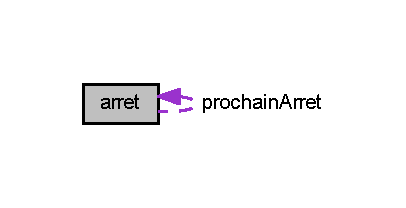
\includegraphics[width=195pt]{classarret__coll__graph}
\end{center}
\end{figure}
\subsection*{Public Member Functions}
\begin{DoxyCompactItemize}
\item 
\hyperlink{classarret_ae38cddedd9355eeaebbafe40bcb4b0bc}{arret} (double \hyperlink{classarret_a10d9c6ad4411da3b31072f04633745d1}{posX}, double \hyperlink{classarret_a87be7e932dbc73b03ba64969c1413faa}{posY}, int \hyperlink{classarret_afc7a6e7cb0cb73e242a4c6ad8743995c}{temps\+Arret}, std\+::string \hyperlink{classarret_a543d7100f999b9f0267945bf44c67d4b}{nom\+Arret})
\end{DoxyCompactItemize}
\subsection*{Public Attributes}
\begin{DoxyCompactItemize}
\item 
\hyperlink{classarret}{arret} $\ast$ \hyperlink{classarret_a69ca61ad6399a414b15a2bcc1cc4a81c}{prochain\+Arret}
\item 
double \hyperlink{classarret_a10d9c6ad4411da3b31072f04633745d1}{posX}
\item 
double \hyperlink{classarret_a87be7e932dbc73b03ba64969c1413faa}{posY}
\item 
int \hyperlink{classarret_afc7a6e7cb0cb73e242a4c6ad8743995c}{temps\+Arret}
\item 
std\+::string \hyperlink{classarret_a543d7100f999b9f0267945bf44c67d4b}{nom\+Arret}
\item 
int \hyperlink{classarret_aff9a2ea0c2261ea5ea0c04e5b84880bb}{num\+Trams\+Sur\+Place}
\end{DoxyCompactItemize}
\subsection*{Friends}
\begin{DoxyCompactItemize}
\item 
class \hyperlink{classarret_af9ab36d65ca58c516f6f72ca840ebd7b}{liste\+Arrets}
\end{DoxyCompactItemize}


\subsection{Constructor \& Destructor Documentation}
\index{arret@{arret}!arret@{arret}}
\index{arret@{arret}!arret@{arret}}
\subsubsection[{\texorpdfstring{arret(double pos\+X, double pos\+Y, int temps\+Arret, std\+::string nom\+Arret)}{arret(double posX, double posY, int tempsArret, std::string nomArret)}}]{\setlength{\rightskip}{0pt plus 5cm}arret\+::arret (
\begin{DoxyParamCaption}
\item[{double}]{posX, }
\item[{double}]{posY, }
\item[{int}]{temps\+Arret, }
\item[{std\+::string}]{nom\+Arret}
\end{DoxyParamCaption}
)}\hypertarget{classarret_ae38cddedd9355eeaebbafe40bcb4b0bc}{}\label{classarret_ae38cddedd9355eeaebbafe40bcb4b0bc}
Constructeur d\textquotesingle{}arret 
\begin{DoxyParams}[1]{Parameters}
\mbox{\tt in}  & {\em posX} & -\/ \\
\hline
\mbox{\tt in}  & {\em posY} & -\/ \\
\hline
\mbox{\tt in}  & {\em temps\+Arret} & -\/ \\
\hline
\mbox{\tt in}  & {\em nom\+Arret} & -\/ \\
\hline
\end{DoxyParams}


\subsection{Friends And Related Function Documentation}
\index{arret@{arret}!liste\+Arrets@{liste\+Arrets}}
\index{liste\+Arrets@{liste\+Arrets}!arret@{arret}}
\subsubsection[{\texorpdfstring{liste\+Arrets}{listeArrets}}]{\setlength{\rightskip}{0pt plus 5cm}friend class {\bf liste\+Arrets}\hspace{0.3cm}{\ttfamily [friend]}}\hypertarget{classarret_af9ab36d65ca58c516f6f72ca840ebd7b}{}\label{classarret_af9ab36d65ca58c516f6f72ca840ebd7b}


\subsection{Member Data Documentation}
\index{arret@{arret}!nom\+Arret@{nom\+Arret}}
\index{nom\+Arret@{nom\+Arret}!arret@{arret}}
\subsubsection[{\texorpdfstring{nom\+Arret}{nomArret}}]{\setlength{\rightskip}{0pt plus 5cm}std\+::string arret\+::nom\+Arret}\hypertarget{classarret_a543d7100f999b9f0267945bf44c67d4b}{}\label{classarret_a543d7100f999b9f0267945bf44c67d4b}
\index{arret@{arret}!num\+Trams\+Sur\+Place@{num\+Trams\+Sur\+Place}}
\index{num\+Trams\+Sur\+Place@{num\+Trams\+Sur\+Place}!arret@{arret}}
\subsubsection[{\texorpdfstring{num\+Trams\+Sur\+Place}{numTramsSurPlace}}]{\setlength{\rightskip}{0pt plus 5cm}int arret\+::num\+Trams\+Sur\+Place}\hypertarget{classarret_aff9a2ea0c2261ea5ea0c04e5b84880bb}{}\label{classarret_aff9a2ea0c2261ea5ea0c04e5b84880bb}
\index{arret@{arret}!posX@{posX}}
\index{posX@{posX}!arret@{arret}}
\subsubsection[{\texorpdfstring{posX}{posX}}]{\setlength{\rightskip}{0pt plus 5cm}double arret\+::posX}\hypertarget{classarret_a10d9c6ad4411da3b31072f04633745d1}{}\label{classarret_a10d9c6ad4411da3b31072f04633745d1}
\index{arret@{arret}!posY@{posY}}
\index{posY@{posY}!arret@{arret}}
\subsubsection[{\texorpdfstring{posY}{posY}}]{\setlength{\rightskip}{0pt plus 5cm}double arret\+::posY}\hypertarget{classarret_a87be7e932dbc73b03ba64969c1413faa}{}\label{classarret_a87be7e932dbc73b03ba64969c1413faa}
\index{arret@{arret}!prochain\+Arret@{prochain\+Arret}}
\index{prochain\+Arret@{prochain\+Arret}!arret@{arret}}
\subsubsection[{\texorpdfstring{prochain\+Arret}{prochainArret}}]{\setlength{\rightskip}{0pt plus 5cm}{\bf arret}$\ast$ arret\+::prochain\+Arret}\hypertarget{classarret_a69ca61ad6399a414b15a2bcc1cc4a81c}{}\label{classarret_a69ca61ad6399a414b15a2bcc1cc4a81c}
\index{arret@{arret}!temps\+Arret@{temps\+Arret}}
\index{temps\+Arret@{temps\+Arret}!arret@{arret}}
\subsubsection[{\texorpdfstring{temps\+Arret}{tempsArret}}]{\setlength{\rightskip}{0pt plus 5cm}int arret\+::temps\+Arret}\hypertarget{classarret_afc7a6e7cb0cb73e242a4c6ad8743995c}{}\label{classarret_afc7a6e7cb0cb73e242a4c6ad8743995c}


The documentation for this class was generated from the following files\+:\begin{DoxyCompactItemize}
\item 
C\+:/\+Users/oumar12/\+Desktop/\+T\+R\+A\+M\+W\+A\+Y\+S/\+T\+R\+A\+M\+W\+A\+Y\+S/\hyperlink{liste_arrets_8h}{liste\+Arrets.\+h}\item 
C\+:/\+Users/oumar12/\+Desktop/\+T\+R\+A\+M\+W\+A\+Y\+S/\+T\+R\+A\+M\+W\+A\+Y\+S/\hyperlink{liste_arrets_8cpp}{liste\+Arrets.\+cpp}\end{DoxyCompactItemize}

\hypertarget{classlecture_x_m_l}{}\section{lecture\+X\+ML Class Reference}
\label{classlecture_x_m_l}\index{lecture\+X\+ML@{lecture\+X\+ML}}


{\ttfamily \#include $<$lecture\+X\+M\+L.\+h$>$}

\subsection*{Public Member Functions}
\begin{DoxyCompactItemize}
\item 
\hyperlink{classlecture_x_m_l_a1143069c6b2231c9a3d46411e29f1ca0}{lecture\+X\+ML} (std\+::string nom\+Fichier, int temps)
\end{DoxyCompactItemize}


\subsection{Constructor \& Destructor Documentation}
\index{lecture\+X\+ML@{lecture\+X\+ML}!lecture\+X\+ML@{lecture\+X\+ML}}
\index{lecture\+X\+ML@{lecture\+X\+ML}!lecture\+X\+ML@{lecture\+X\+ML}}
\subsubsection[{\texorpdfstring{lecture\+X\+M\+L(std\+::string nom\+Fichier, int temps)}{lectureXML(std::string nomFichier, int temps)}}]{\setlength{\rightskip}{0pt plus 5cm}lecture\+X\+M\+L\+::lecture\+X\+ML (
\begin{DoxyParamCaption}
\item[{std\+::string}]{nom\+Fichier, }
\item[{int}]{temps}
\end{DoxyParamCaption}
)}\hypertarget{classlecture_x_m_l_a1143069c6b2231c9a3d46411e29f1ca0}{}\label{classlecture_x_m_l_a1143069c6b2231c9a3d46411e29f1ca0}
Permet de lire un fichier X\+ML. 
\begin{DoxyParams}[1]{Parameters}
\mbox{\tt in}  & {\em nom\+Fichier} & -\/ nom du fichier \\
\hline
\mbox{\tt in}  & {\em temps} & -\/ temps d\textquotesingle{}execution \\
\hline
\end{DoxyParams}


Here is the call graph for this function\+:
\nopagebreak
\begin{figure}[H]
\begin{center}
\leavevmode
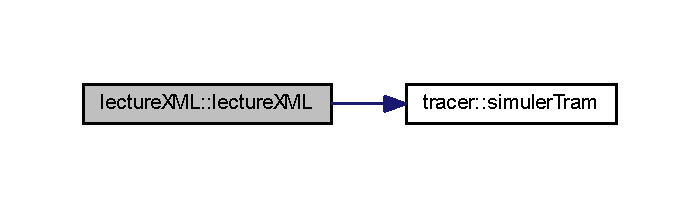
\includegraphics[width=336pt]{classlecture_x_m_l_a1143069c6b2231c9a3d46411e29f1ca0_cgraph}
\end{center}
\end{figure}




The documentation for this class was generated from the following files\+:\begin{DoxyCompactItemize}
\item 
C\+:/\+Users/oumar12/\+Desktop/\+T\+R\+A\+M\+W\+A\+Y\+S/\+T\+R\+A\+M\+W\+A\+Y\+S/\hyperlink{lecture_x_m_l_8h}{lecture\+X\+M\+L.\+h}\item 
C\+:/\+Users/oumar12/\+Desktop/\+T\+R\+A\+M\+W\+A\+Y\+S/\+T\+R\+A\+M\+W\+A\+Y\+S/\hyperlink{lecture_x_m_l_8cpp}{lecture\+X\+M\+L.\+cpp}\end{DoxyCompactItemize}

\hypertarget{classligne}{}\section{ligne Class Reference}
\label{classligne}\index{ligne@{ligne}}


{\ttfamily \#include $<$ligne.\+h$>$}

\subsection*{Public Member Functions}
\begin{DoxyCompactItemize}
\item 
\hyperlink{classligne_ab9ab2dab09a1d5335f0f33911a5f0fdf}{ligne} ()
\begin{DoxyCompactList}\small\item\em Constructeur par default. \end{DoxyCompactList}\item 
\hyperlink{classligne_a46cce30fd93232136e89005a3a46327a}{ligne} (int \hyperlink{classligne_abc5c8d7ccfe9aedc12ccd58d8d5f2cb4}{num\+De\+Ligne}, std\+::string \hyperlink{classligne_adef9f7b87df4ee2a16becd9ca1cd81b0}{nom\+De\+Ligne}, double \hyperlink{classligne_a68736df5931bd7755dc3b5c19950576f}{distance\+Entre\+Arrets}, \hyperlink{classliste_arrets}{liste\+Arrets} $\ast$\hyperlink{classligne_a46e5f1af388d0c918333427098898d8b}{arrets}, \hyperlink{classliste_de_trams}{liste\+De\+Trams} $\ast$\hyperlink{classligne_a5f373b366977d04b0e2eaf8bf32c6036}{trams})
\item 
\hyperlink{classligne_a2ef56d3dcf06db6971c2d44cb73ba8ad}{ligne} (\hyperlink{classligne}{ligne} $\ast$ligne\+\_\+a\+\_\+\+Creer)
\item 
std\+::string \hyperlink{classligne_adef9f7b87df4ee2a16becd9ca1cd81b0}{nom\+De\+Ligne} () const 
\begin{DoxyCompactList}\small\item\em Methodes Acc�s \end{DoxyCompactList}\item 
int \hyperlink{classligne_abc5c8d7ccfe9aedc12ccd58d8d5f2cb4}{num\+De\+Ligne} () const 
\item 
\hyperlink{classliste_arrets}{liste\+Arrets} $\ast$ \hyperlink{classligne_a46e5f1af388d0c918333427098898d8b}{arrets} () const 
\item 
\hyperlink{classliste_de_trams}{liste\+De\+Trams} $\ast$ \hyperlink{classligne_a5f373b366977d04b0e2eaf8bf32c6036}{trams} () const 
\item 
double \hyperlink{classligne_a68736df5931bd7755dc3b5c19950576f}{distance\+Entre\+Arrets} () const 
\item 
void \hyperlink{classligne_a7da92f90eb4c91c1b5446039032c298f}{nom\+De\+Ligne} (std\+::string nom\+De\+Ligne)
\begin{DoxyCompactList}\small\item\em Methodes de modification. \end{DoxyCompactList}\item 
void \hyperlink{classligne_aa83ea0670f7d31f947dbb5fd678dc847}{num\+De\+Ligne} (int num\+De\+Ligne)
\item 
void \hyperlink{classligne_a1128030fba3430f9a365f670cbd461dc}{arrets} (\hyperlink{classliste_arrets}{liste\+Arrets} $\ast$arrets)
\item 
void \hyperlink{classligne_a5cde292801e3554a0bffd35ce83c49be}{trams} (\hyperlink{classliste_de_trams}{liste\+De\+Trams} $\ast$trams)
\item 
void \hyperlink{classligne_ad4157a1b708436c8f07f262f1aa2b3d6}{distance\+Entre\+Arrets} (double distance\+Entre\+Arrets)
\item 
\hyperlink{classligne_ab282119bfd4ad9d32620735056ad3dac}{$\sim$ligne} ()
\begin{DoxyCompactList}\small\item\em Destructeur. \end{DoxyCompactList}\end{DoxyCompactItemize}


\subsection{Constructor \& Destructor Documentation}
\index{ligne@{ligne}!ligne@{ligne}}
\index{ligne@{ligne}!ligne@{ligne}}
\subsubsection[{\texorpdfstring{ligne()}{ligne()}}]{\setlength{\rightskip}{0pt plus 5cm}ligne\+::ligne (
\begin{DoxyParamCaption}
{}
\end{DoxyParamCaption}
)}\hypertarget{classligne_ab9ab2dab09a1d5335f0f33911a5f0fdf}{}\label{classligne_ab9ab2dab09a1d5335f0f33911a5f0fdf}


Constructeur par default. 

\index{ligne@{ligne}!ligne@{ligne}}
\index{ligne@{ligne}!ligne@{ligne}}
\subsubsection[{\texorpdfstring{ligne(int num\+De\+Ligne, std\+::string nom\+De\+Ligne, double distance\+Entre\+Arrets, liste\+Arrets $\ast$arrets, liste\+De\+Trams $\ast$trams)}{ligne(int numDeLigne, std::string nomDeLigne, double distanceEntreArrets, listeArrets *arrets, listeDeTrams *trams)}}]{\setlength{\rightskip}{0pt plus 5cm}ligne\+::ligne (
\begin{DoxyParamCaption}
\item[{int}]{num\+De\+Ligne, }
\item[{std\+::string}]{nom\+De\+Ligne, }
\item[{double}]{distance\+Entre\+Arrets, }
\item[{{\bf liste\+Arrets} $\ast$}]{arrets, }
\item[{{\bf liste\+De\+Trams} $\ast$}]{trams}
\end{DoxyParamCaption}
)}\hypertarget{classligne_a46cce30fd93232136e89005a3a46327a}{}\label{classligne_a46cce30fd93232136e89005a3a46327a}
Constructeur par d�faut 
\begin{DoxyParams}[1]{Parameters}
\mbox{\tt in}  & {\em num\+Ligne} & -\/ numero de ligne \\
\hline
\mbox{\tt in}  & {\em nom\+Ligne} & -\/ nom de ligne \\
\hline
\mbox{\tt in}  & {\em arrets} & -\/ liste des arrets \\
\hline
\mbox{\tt in}  & {\em trams} & -\/ listes des trams \\
\hline
\mbox{\tt in}  & {\em distance\+Arret} & -\/ distance entre chaque arret \\
\hline
\end{DoxyParams}


Here is the call graph for this function\+:
\nopagebreak
\begin{figure}[H]
\begin{center}
\leavevmode
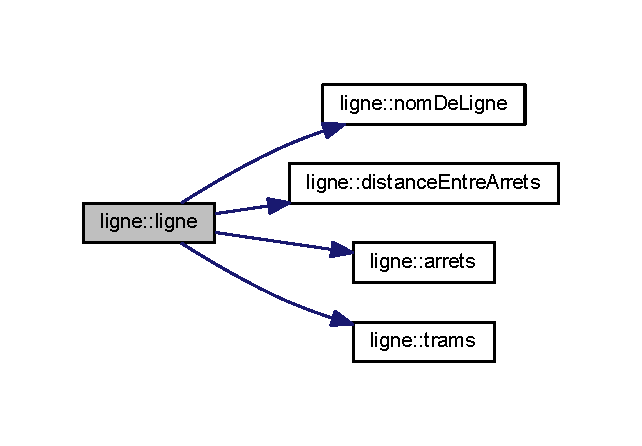
\includegraphics[width=308pt]{classligne_a46cce30fd93232136e89005a3a46327a_cgraph}
\end{center}
\end{figure}


\index{ligne@{ligne}!ligne@{ligne}}
\index{ligne@{ligne}!ligne@{ligne}}
\subsubsection[{\texorpdfstring{ligne(ligne $\ast$ligne\+\_\+a\+\_\+\+Creer)}{ligne(ligne *ligne_a_Creer)}}]{\setlength{\rightskip}{0pt plus 5cm}ligne\+::ligne (
\begin{DoxyParamCaption}
\item[{{\bf ligne} $\ast$}]{ligne\+\_\+a\+\_\+\+Creer}
\end{DoxyParamCaption}
)}\hypertarget{classligne_a2ef56d3dcf06db6971c2d44cb73ba8ad}{}\label{classligne_a2ef56d3dcf06db6971c2d44cb73ba8ad}
Constructeur par ligne 
\begin{DoxyParams}[1]{Parameters}
\mbox{\tt in}  & {\em maligne} & -\/ ligne � cr�e \\
\hline
\end{DoxyParams}


Here is the call graph for this function\+:
\nopagebreak
\begin{figure}[H]
\begin{center}
\leavevmode
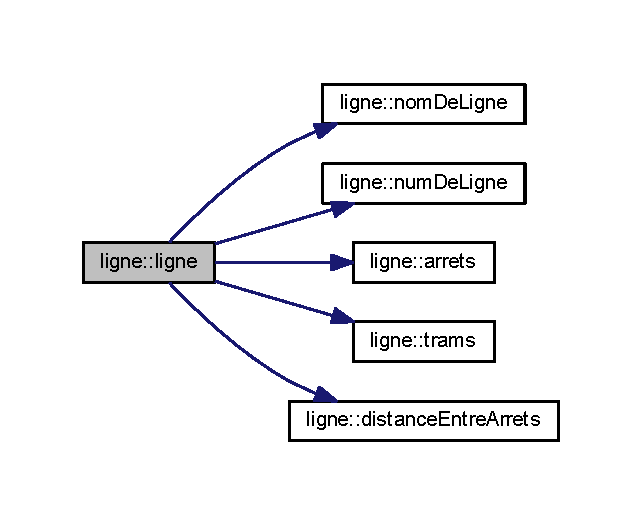
\includegraphics[width=308pt]{classligne_a2ef56d3dcf06db6971c2d44cb73ba8ad_cgraph}
\end{center}
\end{figure}


\index{ligne@{ligne}!````~ligne@{$\sim$ligne}}
\index{````~ligne@{$\sim$ligne}!ligne@{ligne}}
\subsubsection[{\texorpdfstring{$\sim$ligne()}{~ligne()}}]{\setlength{\rightskip}{0pt plus 5cm}ligne\+::$\sim$ligne (
\begin{DoxyParamCaption}
{}
\end{DoxyParamCaption}
)}\hypertarget{classligne_ab282119bfd4ad9d32620735056ad3dac}{}\label{classligne_ab282119bfd4ad9d32620735056ad3dac}


Destructeur. 



\subsection{Member Function Documentation}
\index{ligne@{ligne}!arrets@{arrets}}
\index{arrets@{arrets}!ligne@{ligne}}
\subsubsection[{\texorpdfstring{arrets() const }{arrets() const }}]{\setlength{\rightskip}{0pt plus 5cm}{\bf liste\+Arrets} $\ast$ ligne\+::arrets (
\begin{DoxyParamCaption}
{}
\end{DoxyParamCaption}
) const}\hypertarget{classligne_a46e5f1af388d0c918333427098898d8b}{}\label{classligne_a46e5f1af388d0c918333427098898d8b}
\begin{DoxyReturn}{Returns}
-\/ return un private d\+\_\+arrets 
\end{DoxyReturn}


Here is the caller graph for this function\+:
\nopagebreak
\begin{figure}[H]
\begin{center}
\leavevmode
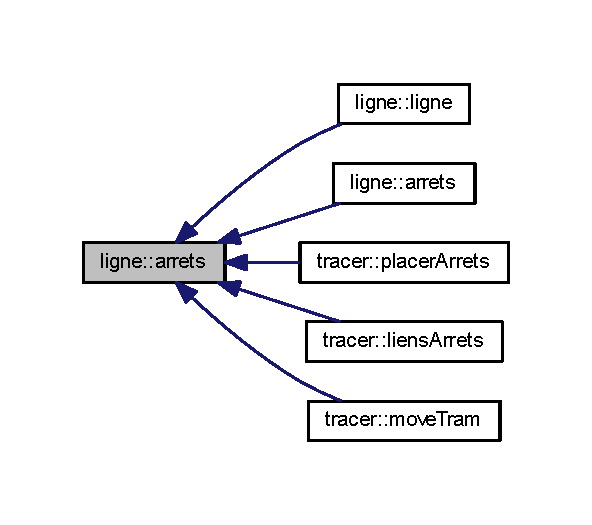
\includegraphics[width=284pt]{classligne_a46e5f1af388d0c918333427098898d8b_icgraph}
\end{center}
\end{figure}


\index{ligne@{ligne}!arrets@{arrets}}
\index{arrets@{arrets}!ligne@{ligne}}
\subsubsection[{\texorpdfstring{arrets(liste\+Arrets $\ast$arrets)}{arrets(listeArrets *arrets)}}]{\setlength{\rightskip}{0pt plus 5cm}void ligne\+::arrets (
\begin{DoxyParamCaption}
\item[{{\bf liste\+Arrets} $\ast$}]{arrets}
\end{DoxyParamCaption}
)}\hypertarget{classligne_a1128030fba3430f9a365f670cbd461dc}{}\label{classligne_a1128030fba3430f9a365f670cbd461dc}

\begin{DoxyParams}[1]{Parameters}
\mbox{\tt in}  & {\em arrets} & -\/ liste des arrets \\
\hline
\end{DoxyParams}


Here is the call graph for this function\+:
\nopagebreak
\begin{figure}[H]
\begin{center}
\leavevmode
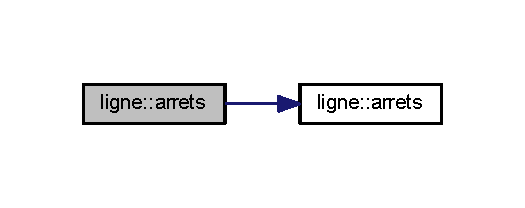
\includegraphics[width=252pt]{classligne_a1128030fba3430f9a365f670cbd461dc_cgraph}
\end{center}
\end{figure}


\index{ligne@{ligne}!distance\+Entre\+Arrets@{distance\+Entre\+Arrets}}
\index{distance\+Entre\+Arrets@{distance\+Entre\+Arrets}!ligne@{ligne}}
\subsubsection[{\texorpdfstring{distance\+Entre\+Arrets() const }{distanceEntreArrets() const }}]{\setlength{\rightskip}{0pt plus 5cm}double ligne\+::distance\+Entre\+Arrets (
\begin{DoxyParamCaption}
{}
\end{DoxyParamCaption}
) const}\hypertarget{classligne_a68736df5931bd7755dc3b5c19950576f}{}\label{classligne_a68736df5931bd7755dc3b5c19950576f}
\begin{DoxyReturn}{Returns}
-\/ return un private d\+\_\+distance\+Entr\+Arrets 
\end{DoxyReturn}


Here is the caller graph for this function\+:
\nopagebreak
\begin{figure}[H]
\begin{center}
\leavevmode
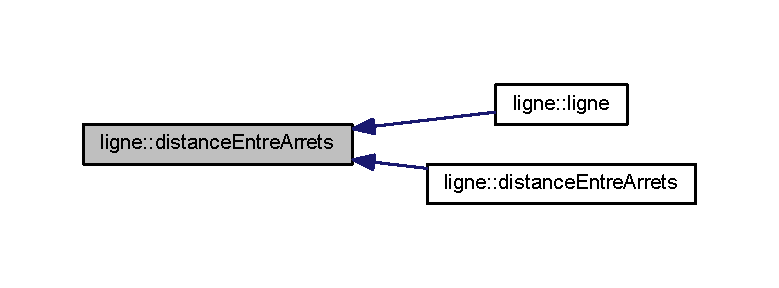
\includegraphics[width=350pt]{classligne_a68736df5931bd7755dc3b5c19950576f_icgraph}
\end{center}
\end{figure}


\index{ligne@{ligne}!distance\+Entre\+Arrets@{distance\+Entre\+Arrets}}
\index{distance\+Entre\+Arrets@{distance\+Entre\+Arrets}!ligne@{ligne}}
\subsubsection[{\texorpdfstring{distance\+Entre\+Arrets(double distance\+Entre\+Arrets)}{distanceEntreArrets(double distanceEntreArrets)}}]{\setlength{\rightskip}{0pt plus 5cm}void ligne\+::distance\+Entre\+Arrets (
\begin{DoxyParamCaption}
\item[{double}]{distance\+Entre\+Arrets}
\end{DoxyParamCaption}
)}\hypertarget{classligne_ad4157a1b708436c8f07f262f1aa2b3d6}{}\label{classligne_ad4157a1b708436c8f07f262f1aa2b3d6}

\begin{DoxyParams}[1]{Parameters}
\mbox{\tt in}  & {\em distance\+Entre\+Arrets} & -\/ distance entre les arrets \\
\hline
\end{DoxyParams}


Here is the call graph for this function\+:
\nopagebreak
\begin{figure}[H]
\begin{center}
\leavevmode
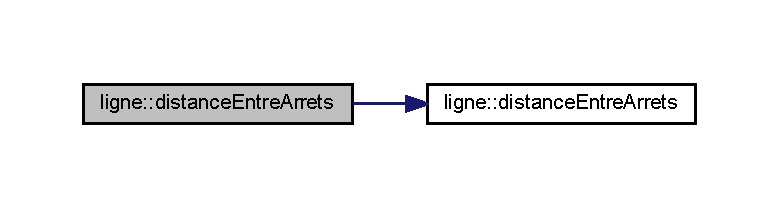
\includegraphics[width=350pt]{classligne_ad4157a1b708436c8f07f262f1aa2b3d6_cgraph}
\end{center}
\end{figure}


\index{ligne@{ligne}!nom\+De\+Ligne@{nom\+De\+Ligne}}
\index{nom\+De\+Ligne@{nom\+De\+Ligne}!ligne@{ligne}}
\subsubsection[{\texorpdfstring{nom\+De\+Ligne() const }{nomDeLigne() const }}]{\setlength{\rightskip}{0pt plus 5cm}std\+::string ligne\+::nom\+De\+Ligne (
\begin{DoxyParamCaption}
{}
\end{DoxyParamCaption}
) const}\hypertarget{classligne_adef9f7b87df4ee2a16becd9ca1cd81b0}{}\label{classligne_adef9f7b87df4ee2a16becd9ca1cd81b0}


Methodes Acc�s 

\begin{DoxyReturn}{Returns}
-\/ retourne le nom de la ligne 
\end{DoxyReturn}


Here is the caller graph for this function\+:
\nopagebreak
\begin{figure}[H]
\begin{center}
\leavevmode
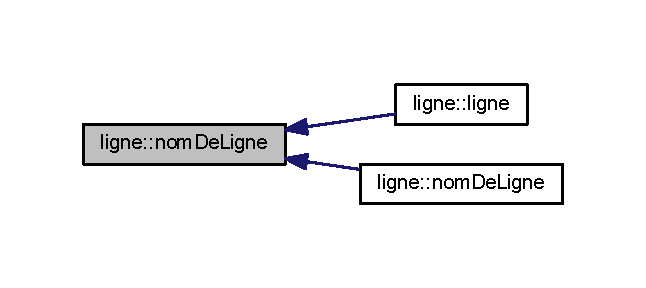
\includegraphics[width=310pt]{classligne_adef9f7b87df4ee2a16becd9ca1cd81b0_icgraph}
\end{center}
\end{figure}


\index{ligne@{ligne}!nom\+De\+Ligne@{nom\+De\+Ligne}}
\index{nom\+De\+Ligne@{nom\+De\+Ligne}!ligne@{ligne}}
\subsubsection[{\texorpdfstring{nom\+De\+Ligne(std\+::string nom\+De\+Ligne)}{nomDeLigne(std::string nomDeLigne)}}]{\setlength{\rightskip}{0pt plus 5cm}void ligne\+::nom\+De\+Ligne (
\begin{DoxyParamCaption}
\item[{std\+::string}]{nom\+De\+Ligne}
\end{DoxyParamCaption}
)}\hypertarget{classligne_a7da92f90eb4c91c1b5446039032c298f}{}\label{classligne_a7da92f90eb4c91c1b5446039032c298f}


Methodes de modification. 


\begin{DoxyParams}[1]{Parameters}
\mbox{\tt in}  & {\em nom\+Ligne} & -\/ nom de ligne \\
\hline
\end{DoxyParams}


Here is the call graph for this function\+:
\nopagebreak
\begin{figure}[H]
\begin{center}
\leavevmode
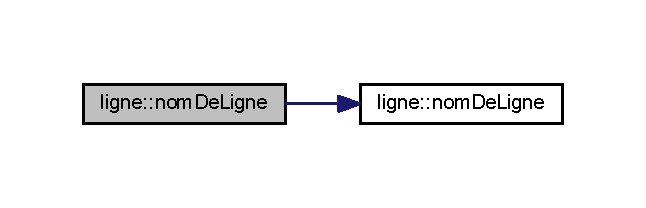
\includegraphics[width=310pt]{classligne_a7da92f90eb4c91c1b5446039032c298f_cgraph}
\end{center}
\end{figure}


\index{ligne@{ligne}!num\+De\+Ligne@{num\+De\+Ligne}}
\index{num\+De\+Ligne@{num\+De\+Ligne}!ligne@{ligne}}
\subsubsection[{\texorpdfstring{num\+De\+Ligne() const }{numDeLigne() const }}]{\setlength{\rightskip}{0pt plus 5cm}int ligne\+::num\+De\+Ligne (
\begin{DoxyParamCaption}
{}
\end{DoxyParamCaption}
) const}\hypertarget{classligne_abc5c8d7ccfe9aedc12ccd58d8d5f2cb4}{}\label{classligne_abc5c8d7ccfe9aedc12ccd58d8d5f2cb4}
\begin{DoxyReturn}{Returns}
-\/ retourne le numero de la ligne 
\end{DoxyReturn}


Here is the caller graph for this function\+:
\nopagebreak
\begin{figure}[H]
\begin{center}
\leavevmode
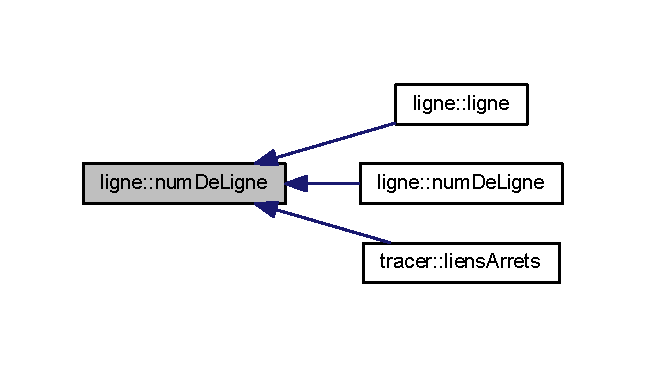
\includegraphics[width=310pt]{classligne_abc5c8d7ccfe9aedc12ccd58d8d5f2cb4_icgraph}
\end{center}
\end{figure}


\index{ligne@{ligne}!num\+De\+Ligne@{num\+De\+Ligne}}
\index{num\+De\+Ligne@{num\+De\+Ligne}!ligne@{ligne}}
\subsubsection[{\texorpdfstring{num\+De\+Ligne(int num\+De\+Ligne)}{numDeLigne(int numDeLigne)}}]{\setlength{\rightskip}{0pt plus 5cm}void ligne\+::num\+De\+Ligne (
\begin{DoxyParamCaption}
\item[{int}]{num\+De\+Ligne}
\end{DoxyParamCaption}
)}\hypertarget{classligne_aa83ea0670f7d31f947dbb5fd678dc847}{}\label{classligne_aa83ea0670f7d31f947dbb5fd678dc847}

\begin{DoxyParams}[1]{Parameters}
\mbox{\tt in}  & {\em num\+De\+Ligne} & -\/ numero de ligne \\
\hline
\end{DoxyParams}


Here is the call graph for this function\+:
\nopagebreak
\begin{figure}[H]
\begin{center}
\leavevmode
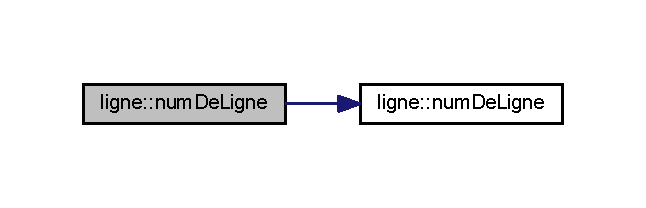
\includegraphics[width=310pt]{classligne_aa83ea0670f7d31f947dbb5fd678dc847_cgraph}
\end{center}
\end{figure}


\index{ligne@{ligne}!trams@{trams}}
\index{trams@{trams}!ligne@{ligne}}
\subsubsection[{\texorpdfstring{trams() const }{trams() const }}]{\setlength{\rightskip}{0pt plus 5cm}{\bf liste\+De\+Trams} $\ast$ ligne\+::trams (
\begin{DoxyParamCaption}
{}
\end{DoxyParamCaption}
) const}\hypertarget{classligne_a5f373b366977d04b0e2eaf8bf32c6036}{}\label{classligne_a5f373b366977d04b0e2eaf8bf32c6036}
\begin{DoxyReturn}{Returns}
-\/ return un private d\+\_\+trams 
\end{DoxyReturn}


Here is the caller graph for this function\+:
\nopagebreak
\begin{figure}[H]
\begin{center}
\leavevmode
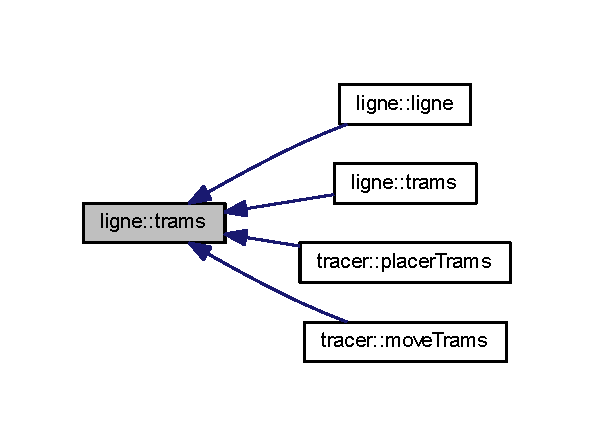
\includegraphics[width=285pt]{classligne_a5f373b366977d04b0e2eaf8bf32c6036_icgraph}
\end{center}
\end{figure}


\index{ligne@{ligne}!trams@{trams}}
\index{trams@{trams}!ligne@{ligne}}
\subsubsection[{\texorpdfstring{trams(liste\+De\+Trams $\ast$trams)}{trams(listeDeTrams *trams)}}]{\setlength{\rightskip}{0pt plus 5cm}void ligne\+::trams (
\begin{DoxyParamCaption}
\item[{{\bf liste\+De\+Trams} $\ast$}]{trams}
\end{DoxyParamCaption}
)}\hypertarget{classligne_a5cde292801e3554a0bffd35ce83c49be}{}\label{classligne_a5cde292801e3554a0bffd35ce83c49be}

\begin{DoxyParams}[1]{Parameters}
\mbox{\tt in}  & {\em trams} & -\/ liste de trams \\
\hline
\end{DoxyParams}


Here is the call graph for this function\+:
\nopagebreak
\begin{figure}[H]
\begin{center}
\leavevmode
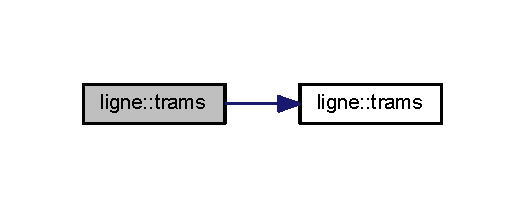
\includegraphics[width=252pt]{classligne_a5cde292801e3554a0bffd35ce83c49be_cgraph}
\end{center}
\end{figure}




The documentation for this class was generated from the following files\+:\begin{DoxyCompactItemize}
\item 
C\+:/\+Users/oumar12/\+Desktop/\+T\+R\+A\+M\+W\+A\+Y\+S/\+T\+R\+A\+M\+W\+A\+Y\+S/\hyperlink{ligne_8h}{ligne.\+h}\item 
C\+:/\+Users/oumar12/\+Desktop/\+T\+R\+A\+M\+W\+A\+Y\+S/\+T\+R\+A\+M\+W\+A\+Y\+S/\hyperlink{ligne_8cpp}{ligne.\+cpp}\end{DoxyCompactItemize}

\hypertarget{classliste_arrets}{}\section{liste\+Arrets Class Reference}
\label{classliste_arrets}\index{liste\+Arrets@{liste\+Arrets}}


{\ttfamily \#include $<$liste\+Arrets.\+h$>$}

\subsection*{Public Member Functions}
\begin{DoxyCompactItemize}
\item 
\hyperlink{classliste_arrets_abbfaa5d64a48879f0786338279371b83}{liste\+Arrets} ()
\begin{DoxyCompactList}\small\item\em Constructeur. \end{DoxyCompactList}\item 
void \hyperlink{classliste_arrets_a7168c4b4ca72f6ab07f02d4af5877586}{ajout\+En\+Tete} (double posX, double posY, int temps\+Arret, std\+::string nom\+Arret)
\begin{DoxyCompactList}\small\item\em A\+J\+O\+U\+TS. \end{DoxyCompactList}\item 
void \hyperlink{classliste_arrets_adbe0e8547d19edc9bf0982296fab2dfe}{ajout\+Au\+Corps} (double posX, double posY, int temps\+Arret, std\+::string nom\+Arret, int corps)
\item 
void \hyperlink{classliste_arrets_ad9ed677ee4b46f66fdfaba2386dd76c0}{ajout\+Au\+Queue} (double posX, double posY, int temps\+Arret, std\+::string nom\+Arret)
\begin{DoxyCompactList}\small\item\em A\+J\+O\+U\+TS. \end{DoxyCompactList}\item 
void \hyperlink{classliste_arrets_a20fce6e1d98821ff429d7f7f3c9884d3}{suppr\+En\+Tete} ()
\begin{DoxyCompactList}\small\item\em S\+U\+P\+P\+R\+I\+M\+ER. \end{DoxyCompactList}\item 
void \hyperlink{classliste_arrets_a41a1078cbefd801be82a355bd3aa7a75}{suppr\+Au\+Corps} (int corps)
\item 
void \hyperlink{classliste_arrets_a2321a82dd320d42c1a448035e0bd80e9}{suppr\+Au\+Queue} ()
\item 
\hyperlink{classarret}{arret} $\ast$ \hyperlink{classliste_arrets_aae9dc33e355d001c9c4dc1646a2f632d}{acces\+En\+Tete} () const 
\begin{DoxyCompactList}\small\item\em A\+C\+C\+ES. \end{DoxyCompactList}\item 
\hyperlink{classarret}{arret} $\ast$ \hyperlink{classliste_arrets_aa9a45866bcc46e69260fdb168cec4407}{acces\+Au\+Corps} (int corps) const 
\item 
\hyperlink{classarret}{arret} $\ast$ \hyperlink{classliste_arrets_a29a7a234c4abe23456cea8d2df1029bf}{acces\+Au\+Queue} () const 
\item 
void \hyperlink{classliste_arrets_a7e7a28f3a13ff29e1b62e5c19751650b}{afficher\+Liste} () const 
\begin{DoxyCompactList}\small\item\em Affiche la liste des arrets au niveau console. \end{DoxyCompactList}\item 
bool \hyperlink{classliste_arrets_a5731637ae9971b0188c3d4122a52b022}{est\+Aucun\+Arret} () const 
\item 
int \hyperlink{classliste_arrets_a8ebe5918ee71e0c09060227253ade9d8}{nombre\+Arrets} () const 
\item 
\hyperlink{classliste_arrets_afdde522c1f07a7bd3b9e3f9dc202c532}{$\sim$liste\+Arrets} ()
\begin{DoxyCompactList}\small\item\em Destructeur. \end{DoxyCompactList}\end{DoxyCompactItemize}


\subsection{Constructor \& Destructor Documentation}
\index{liste\+Arrets@{liste\+Arrets}!liste\+Arrets@{liste\+Arrets}}
\index{liste\+Arrets@{liste\+Arrets}!liste\+Arrets@{liste\+Arrets}}
\subsubsection[{\texorpdfstring{liste\+Arrets()}{listeArrets()}}]{\setlength{\rightskip}{0pt plus 5cm}liste\+Arrets\+::liste\+Arrets (
\begin{DoxyParamCaption}
{}
\end{DoxyParamCaption}
)}\hypertarget{classliste_arrets_abbfaa5d64a48879f0786338279371b83}{}\label{classliste_arrets_abbfaa5d64a48879f0786338279371b83}


Constructeur. 

\index{liste\+Arrets@{liste\+Arrets}!````~liste\+Arrets@{$\sim$liste\+Arrets}}
\index{````~liste\+Arrets@{$\sim$liste\+Arrets}!liste\+Arrets@{liste\+Arrets}}
\subsubsection[{\texorpdfstring{$\sim$liste\+Arrets()}{~listeArrets()}}]{\setlength{\rightskip}{0pt plus 5cm}liste\+Arrets\+::$\sim$liste\+Arrets (
\begin{DoxyParamCaption}
{}
\end{DoxyParamCaption}
)}\hypertarget{classliste_arrets_afdde522c1f07a7bd3b9e3f9dc202c532}{}\label{classliste_arrets_afdde522c1f07a7bd3b9e3f9dc202c532}


Destructeur. 

D\+E\+S\+T\+R\+U\+C\+T\+E\+UR. 

\subsection{Member Function Documentation}
\index{liste\+Arrets@{liste\+Arrets}!acces\+Au\+Corps@{acces\+Au\+Corps}}
\index{acces\+Au\+Corps@{acces\+Au\+Corps}!liste\+Arrets@{liste\+Arrets}}
\subsubsection[{\texorpdfstring{acces\+Au\+Corps(int corps) const }{accesAuCorps(int corps) const }}]{\setlength{\rightskip}{0pt plus 5cm}{\bf arret} $\ast$ liste\+Arrets\+::acces\+Au\+Corps (
\begin{DoxyParamCaption}
\item[{int}]{corps}
\end{DoxyParamCaption}
) const}\hypertarget{classliste_arrets_aa9a45866bcc46e69260fdb168cec4407}{}\label{classliste_arrets_aa9a45866bcc46e69260fdb168cec4407}

\begin{DoxyParams}[1]{Parameters}
\mbox{\tt in}  & {\em -\/} & corps \\
\hline
\end{DoxyParams}
\begin{DoxyReturn}{Returns}
-\/ a une position 
\end{DoxyReturn}


Here is the caller graph for this function\+:
\nopagebreak
\begin{figure}[H]
\begin{center}
\leavevmode
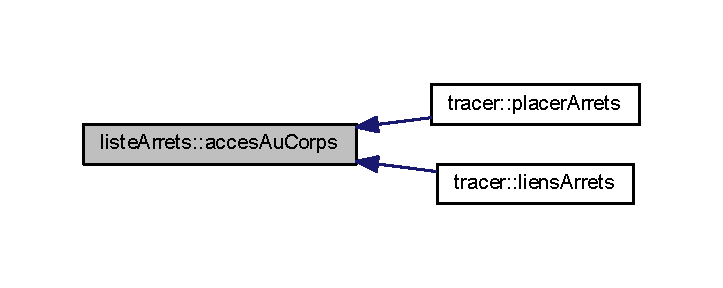
\includegraphics[width=347pt]{classliste_arrets_aa9a45866bcc46e69260fdb168cec4407_icgraph}
\end{center}
\end{figure}


\index{liste\+Arrets@{liste\+Arrets}!acces\+Au\+Queue@{acces\+Au\+Queue}}
\index{acces\+Au\+Queue@{acces\+Au\+Queue}!liste\+Arrets@{liste\+Arrets}}
\subsubsection[{\texorpdfstring{acces\+Au\+Queue() const }{accesAuQueue() const }}]{\setlength{\rightskip}{0pt plus 5cm}{\bf arret} $\ast$ liste\+Arrets\+::acces\+Au\+Queue (
\begin{DoxyParamCaption}
{}
\end{DoxyParamCaption}
) const}\hypertarget{classliste_arrets_a29a7a234c4abe23456cea8d2df1029bf}{}\label{classliste_arrets_a29a7a234c4abe23456cea8d2df1029bf}
\begin{DoxyReturn}{Returns}
-\/ retourne le dernier arret 
\end{DoxyReturn}
\index{liste\+Arrets@{liste\+Arrets}!acces\+En\+Tete@{acces\+En\+Tete}}
\index{acces\+En\+Tete@{acces\+En\+Tete}!liste\+Arrets@{liste\+Arrets}}
\subsubsection[{\texorpdfstring{acces\+En\+Tete() const }{accesEnTete() const }}]{\setlength{\rightskip}{0pt plus 5cm}{\bf arret} $\ast$ liste\+Arrets\+::acces\+En\+Tete (
\begin{DoxyParamCaption}
{}
\end{DoxyParamCaption}
) const}\hypertarget{classliste_arrets_aae9dc33e355d001c9c4dc1646a2f632d}{}\label{classliste_arrets_aae9dc33e355d001c9c4dc1646a2f632d}


A\+C\+C\+ES. 

\begin{DoxyReturn}{Returns}
-\/ le premier arret 
\end{DoxyReturn}


Here is the caller graph for this function\+:
\nopagebreak
\begin{figure}[H]
\begin{center}
\leavevmode
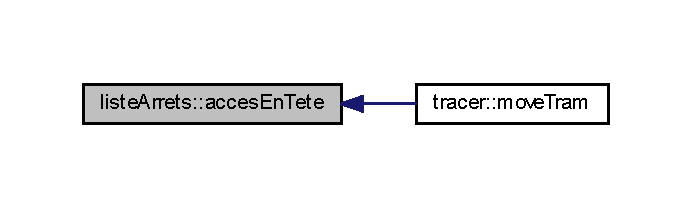
\includegraphics[width=332pt]{classliste_arrets_aae9dc33e355d001c9c4dc1646a2f632d_icgraph}
\end{center}
\end{figure}


\index{liste\+Arrets@{liste\+Arrets}!afficher\+Liste@{afficher\+Liste}}
\index{afficher\+Liste@{afficher\+Liste}!liste\+Arrets@{liste\+Arrets}}
\subsubsection[{\texorpdfstring{afficher\+Liste() const }{afficherListe() const }}]{\setlength{\rightskip}{0pt plus 5cm}void liste\+Arrets\+::afficher\+Liste (
\begin{DoxyParamCaption}
{}
\end{DoxyParamCaption}
) const}\hypertarget{classliste_arrets_a7e7a28f3a13ff29e1b62e5c19751650b}{}\label{classliste_arrets_a7e7a28f3a13ff29e1b62e5c19751650b}


Affiche la liste des arrets au niveau console. 

\index{liste\+Arrets@{liste\+Arrets}!ajout\+Au\+Corps@{ajout\+Au\+Corps}}
\index{ajout\+Au\+Corps@{ajout\+Au\+Corps}!liste\+Arrets@{liste\+Arrets}}
\subsubsection[{\texorpdfstring{ajout\+Au\+Corps(double pos\+X, double pos\+Y, int temps\+Arret, std\+::string nom\+Arret, int corps)}{ajoutAuCorps(double posX, double posY, int tempsArret, std::string nomArret, int corps)}}]{\setlength{\rightskip}{0pt plus 5cm}void liste\+Arrets\+::ajout\+Au\+Corps (
\begin{DoxyParamCaption}
\item[{double}]{posX, }
\item[{double}]{posY, }
\item[{int}]{temps\+Arret, }
\item[{std\+::string}]{nom\+Arret, }
\item[{int}]{corps}
\end{DoxyParamCaption}
)}\hypertarget{classliste_arrets_adbe0e8547d19edc9bf0982296fab2dfe}{}\label{classliste_arrets_adbe0e8547d19edc9bf0982296fab2dfe}

\begin{DoxyParams}[1]{Parameters}
\mbox{\tt in}  & {\em posX} & -\/ \\
\hline
\mbox{\tt in}  & {\em posY} & -\/ \\
\hline
\mbox{\tt in}  & {\em temps\+Arret} & -\/ \\
\hline
\mbox{\tt in}  & {\em nom\+Arret} & -\/ \\
\hline
\mbox{\tt in}  & {\em corsp} & -\/ la position \\
\hline
\end{DoxyParams}


Here is the call graph for this function\+:
\nopagebreak
\begin{figure}[H]
\begin{center}
\leavevmode
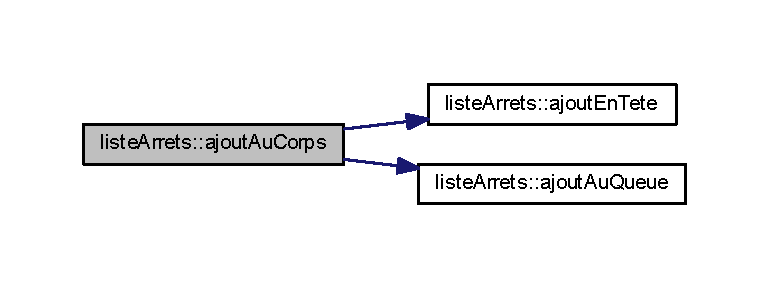
\includegraphics[width=350pt]{classliste_arrets_adbe0e8547d19edc9bf0982296fab2dfe_cgraph}
\end{center}
\end{figure}


\index{liste\+Arrets@{liste\+Arrets}!ajout\+Au\+Queue@{ajout\+Au\+Queue}}
\index{ajout\+Au\+Queue@{ajout\+Au\+Queue}!liste\+Arrets@{liste\+Arrets}}
\subsubsection[{\texorpdfstring{ajout\+Au\+Queue(double pos\+X, double pos\+Y, int temps\+Arret, std\+::string nom\+Arret)}{ajoutAuQueue(double posX, double posY, int tempsArret, std::string nomArret)}}]{\setlength{\rightskip}{0pt plus 5cm}void liste\+Arrets\+::ajout\+Au\+Queue (
\begin{DoxyParamCaption}
\item[{double}]{posX, }
\item[{double}]{posY, }
\item[{int}]{temps\+Arret, }
\item[{std\+::string}]{nom\+Arret}
\end{DoxyParamCaption}
)}\hypertarget{classliste_arrets_ad9ed677ee4b46f66fdfaba2386dd76c0}{}\label{classliste_arrets_ad9ed677ee4b46f66fdfaba2386dd76c0}


A\+J\+O\+U\+TS. 


\begin{DoxyParams}[1]{Parameters}
\mbox{\tt in}  & {\em posX} & -\/ \\
\hline
\mbox{\tt in}  & {\em posY} & -\/ \\
\hline
\mbox{\tt in}  & {\em temps\+Arret} & -\/ \\
\hline
\mbox{\tt in}  & {\em nom\+Arret} & -\/ \\
\hline
\end{DoxyParams}


Here is the caller graph for this function\+:
\nopagebreak
\begin{figure}[H]
\begin{center}
\leavevmode
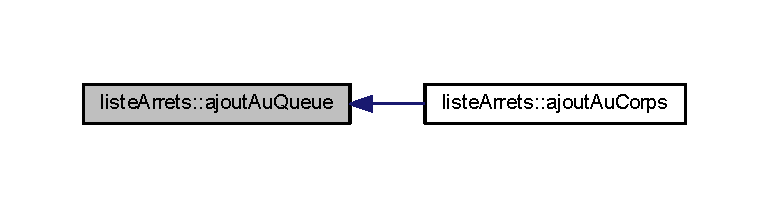
\includegraphics[width=350pt]{classliste_arrets_ad9ed677ee4b46f66fdfaba2386dd76c0_icgraph}
\end{center}
\end{figure}


\index{liste\+Arrets@{liste\+Arrets}!ajout\+En\+Tete@{ajout\+En\+Tete}}
\index{ajout\+En\+Tete@{ajout\+En\+Tete}!liste\+Arrets@{liste\+Arrets}}
\subsubsection[{\texorpdfstring{ajout\+En\+Tete(double pos\+X, double pos\+Y, int temps\+Arret, std\+::string nom\+Arret)}{ajoutEnTete(double posX, double posY, int tempsArret, std::string nomArret)}}]{\setlength{\rightskip}{0pt plus 5cm}void liste\+Arrets\+::ajout\+En\+Tete (
\begin{DoxyParamCaption}
\item[{double}]{posX, }
\item[{double}]{posY, }
\item[{int}]{temps\+Arret, }
\item[{std\+::string}]{nom\+Arret}
\end{DoxyParamCaption}
)}\hypertarget{classliste_arrets_a7168c4b4ca72f6ab07f02d4af5877586}{}\label{classliste_arrets_a7168c4b4ca72f6ab07f02d4af5877586}


A\+J\+O\+U\+TS. 


\begin{DoxyParams}[1]{Parameters}
\mbox{\tt in}  & {\em posX} & -\/ \\
\hline
\mbox{\tt in}  & {\em posY} & -\/ \\
\hline
\mbox{\tt in}  & {\em temps\+Arret} & -\/ \\
\hline
\mbox{\tt in}  & {\em nom\+Arret} & -\/ \\
\hline
\end{DoxyParams}


Here is the caller graph for this function\+:
\nopagebreak
\begin{figure}[H]
\begin{center}
\leavevmode
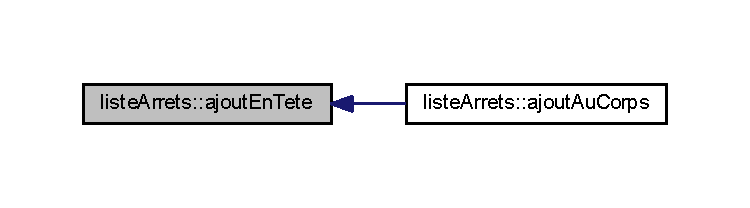
\includegraphics[width=350pt]{classliste_arrets_a7168c4b4ca72f6ab07f02d4af5877586_icgraph}
\end{center}
\end{figure}


\index{liste\+Arrets@{liste\+Arrets}!est\+Aucun\+Arret@{est\+Aucun\+Arret}}
\index{est\+Aucun\+Arret@{est\+Aucun\+Arret}!liste\+Arrets@{liste\+Arrets}}
\subsubsection[{\texorpdfstring{est\+Aucun\+Arret() const }{estAucunArret() const }}]{\setlength{\rightskip}{0pt plus 5cm}bool liste\+Arrets\+::est\+Aucun\+Arret (
\begin{DoxyParamCaption}
{}
\end{DoxyParamCaption}
) const}\hypertarget{classliste_arrets_a5731637ae9971b0188c3d4122a52b022}{}\label{classliste_arrets_a5731637ae9971b0188c3d4122a52b022}
\begin{DoxyReturn}{Returns}
-\/ si le nombre arret est vide 
\end{DoxyReturn}
\index{liste\+Arrets@{liste\+Arrets}!nombre\+Arrets@{nombre\+Arrets}}
\index{nombre\+Arrets@{nombre\+Arrets}!liste\+Arrets@{liste\+Arrets}}
\subsubsection[{\texorpdfstring{nombre\+Arrets() const }{nombreArrets() const }}]{\setlength{\rightskip}{0pt plus 5cm}int liste\+Arrets\+::nombre\+Arrets (
\begin{DoxyParamCaption}
{}
\end{DoxyParamCaption}
) const}\hypertarget{classliste_arrets_a8ebe5918ee71e0c09060227253ade9d8}{}\label{classliste_arrets_a8ebe5918ee71e0c09060227253ade9d8}
\begin{DoxyReturn}{Returns}
-\/ le nombre d\textquotesingle{}arrets 
\end{DoxyReturn}


Here is the caller graph for this function\+:
\nopagebreak
\begin{figure}[H]
\begin{center}
\leavevmode
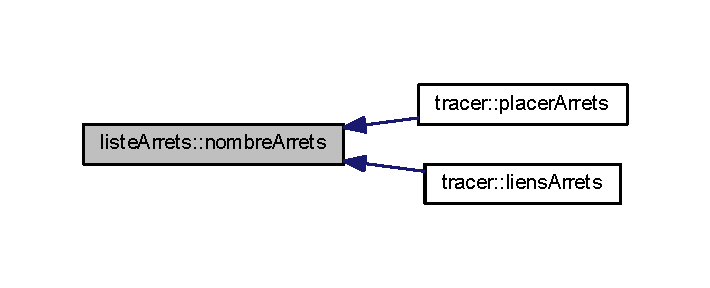
\includegraphics[width=341pt]{classliste_arrets_a8ebe5918ee71e0c09060227253ade9d8_icgraph}
\end{center}
\end{figure}


\index{liste\+Arrets@{liste\+Arrets}!suppr\+Au\+Corps@{suppr\+Au\+Corps}}
\index{suppr\+Au\+Corps@{suppr\+Au\+Corps}!liste\+Arrets@{liste\+Arrets}}
\subsubsection[{\texorpdfstring{suppr\+Au\+Corps(int corps)}{supprAuCorps(int corps)}}]{\setlength{\rightskip}{0pt plus 5cm}void liste\+Arrets\+::suppr\+Au\+Corps (
\begin{DoxyParamCaption}
\item[{int}]{corps}
\end{DoxyParamCaption}
)}\hypertarget{classliste_arrets_a41a1078cbefd801be82a355bd3aa7a75}{}\label{classliste_arrets_a41a1078cbefd801be82a355bd3aa7a75}

\begin{DoxyParams}[1]{Parameters}
\mbox{\tt in}  & {\em -\/} & corps -\/supprimer a une position \\
\hline
\end{DoxyParams}


Here is the call graph for this function\+:
\nopagebreak
\begin{figure}[H]
\begin{center}
\leavevmode
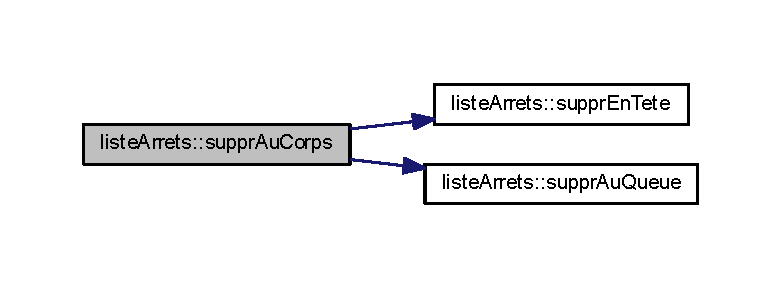
\includegraphics[width=350pt]{classliste_arrets_a41a1078cbefd801be82a355bd3aa7a75_cgraph}
\end{center}
\end{figure}


\index{liste\+Arrets@{liste\+Arrets}!suppr\+Au\+Queue@{suppr\+Au\+Queue}}
\index{suppr\+Au\+Queue@{suppr\+Au\+Queue}!liste\+Arrets@{liste\+Arrets}}
\subsubsection[{\texorpdfstring{suppr\+Au\+Queue()}{supprAuQueue()}}]{\setlength{\rightskip}{0pt plus 5cm}void liste\+Arrets\+::suppr\+Au\+Queue (
\begin{DoxyParamCaption}
{}
\end{DoxyParamCaption}
)}\hypertarget{classliste_arrets_a2321a82dd320d42c1a448035e0bd80e9}{}\label{classliste_arrets_a2321a82dd320d42c1a448035e0bd80e9}
delete au queue 

Here is the caller graph for this function\+:
\nopagebreak
\begin{figure}[H]
\begin{center}
\leavevmode
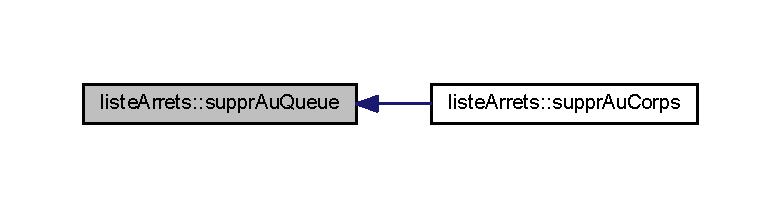
\includegraphics[width=350pt]{classliste_arrets_a2321a82dd320d42c1a448035e0bd80e9_icgraph}
\end{center}
\end{figure}


\index{liste\+Arrets@{liste\+Arrets}!suppr\+En\+Tete@{suppr\+En\+Tete}}
\index{suppr\+En\+Tete@{suppr\+En\+Tete}!liste\+Arrets@{liste\+Arrets}}
\subsubsection[{\texorpdfstring{suppr\+En\+Tete()}{supprEnTete()}}]{\setlength{\rightskip}{0pt plus 5cm}void liste\+Arrets\+::suppr\+En\+Tete (
\begin{DoxyParamCaption}
{}
\end{DoxyParamCaption}
)}\hypertarget{classliste_arrets_a20fce6e1d98821ff429d7f7f3c9884d3}{}\label{classliste_arrets_a20fce6e1d98821ff429d7f7f3c9884d3}


S\+U\+P\+P\+R\+I\+M\+ER. 

S\+U\+P\+P\+R\+E\+S\+S\+I\+ON.

Delete en tete 

Here is the caller graph for this function\+:
\nopagebreak
\begin{figure}[H]
\begin{center}
\leavevmode
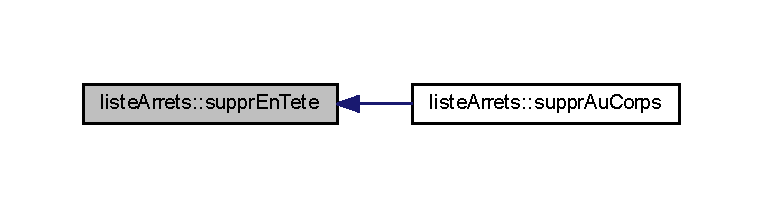
\includegraphics[width=350pt]{classliste_arrets_a20fce6e1d98821ff429d7f7f3c9884d3_icgraph}
\end{center}
\end{figure}




The documentation for this class was generated from the following files\+:\begin{DoxyCompactItemize}
\item 
C\+:/\+Users/oumar12/\+Desktop/\+T\+R\+A\+M\+W\+A\+Y\+S/\+T\+R\+A\+M\+W\+A\+Y\+S/\hyperlink{liste_arrets_8h}{liste\+Arrets.\+h}\item 
C\+:/\+Users/oumar12/\+Desktop/\+T\+R\+A\+M\+W\+A\+Y\+S/\+T\+R\+A\+M\+W\+A\+Y\+S/\hyperlink{liste_arrets_8cpp}{liste\+Arrets.\+cpp}\end{DoxyCompactItemize}

\hypertarget{classliste_de_trams}{}\section{liste\+De\+Trams Class Reference}
\label{classliste_de_trams}\index{liste\+De\+Trams@{liste\+De\+Trams}}


{\ttfamily \#include $<$liste\+De\+Tramway.\+h$>$}

\subsection*{Public Member Functions}
\begin{DoxyCompactItemize}
\item 
\hyperlink{classliste_de_trams_a63cd8796fa2fd5b877f378b1c4e8d66d}{liste\+De\+Trams} ()
\item 
\hyperlink{classliste_de_trams_ac4f850a2d93ad983b485cfa83fdcb57d}{$\sim$liste\+De\+Trams} ()
\begin{DoxyCompactList}\small\item\em D\+E\+S\+T\+R\+U\+C\+T\+E\+UR. \end{DoxyCompactList}\item 
void \hyperlink{classliste_de_trams_acc9f9a3e125a1801cfe108a4a9b27cfc}{ajout\+En\+Tete} (int numero, int vitesse\+Max, bool sens, double posX, double posY, \hyperlink{classligne}{ligne} $\ast$ligne\+Affect)
\begin{DoxyCompactList}\small\item\em A\+J\+O\+U\+TS. \end{DoxyCompactList}\item 
void \hyperlink{classliste_de_trams_af969635f70bda1d3b429a1220e649d7c}{ajout\+Au\+Queue} (int numero, int vitesse\+Max, bool sens, double posX, double posY, \hyperlink{classligne}{ligne} $\ast$ligne\+Affect)
\item 
void \hyperlink{classliste_de_trams_aae576aa98d9709644fee9dda66ea54f7}{ajout\+Au\+Corps} (int numero, int vitesse\+Max, bool sens, double posX, double posY, \hyperlink{classligne}{ligne} $\ast$ligne\+Affect, int corps)
\item 
void \hyperlink{classliste_de_trams_a495cc9d541621a18e3c10817e62d31bd}{suppr\+En\+Tete} ()
\begin{DoxyCompactList}\small\item\em S\+U\+P\+P\+R\+E\+S\+S\+I\+O\+NS. \end{DoxyCompactList}\item 
void \hyperlink{classliste_de_trams_aea83e66431a0a5ff31a631a04f3284cc}{suppr\+Au\+Queue} ()
\item 
void \hyperlink{classliste_de_trams_a718310361597fbe63375c37f3028defa}{suppr\+Au\+Corps} (int corps)
\item 
\hyperlink{classtramway}{tramway} $\ast$ \hyperlink{classliste_de_trams_aa494f9ab59eb0250608782b536f2aa5f}{acces\+En\+Tete} () const 
\begin{DoxyCompactList}\small\item\em A\+C\+C\+ES. \end{DoxyCompactList}\item 
\hyperlink{classtramway}{tramway} $\ast$ \hyperlink{classliste_de_trams_a442cc0dc48c4d8abfd3e8de30a85e24c}{acces\+Au\+Queue} () const 
\item 
\hyperlink{classtramway}{tramway} $\ast$ \hyperlink{classliste_de_trams_a2e66b663287f770c709c16d89424818e}{acces\+Au\+Corps} (int corps) const 
\item 
void \hyperlink{classliste_de_trams_ab1d9638e4f071077f5182413ae8b1c8c}{afficher\+Liste} () const 
\item 
bool \hyperlink{classliste_de_trams_a137520c68e8c14b3cbfa1711d21849a1}{est\+Vide} () const 
\item 
int \hyperlink{classliste_de_trams_afd3b9e87aa935dca81ce3f6d1aea6f75}{nombre\+De\+Trams} () const 
\end{DoxyCompactItemize}


\subsection{Constructor \& Destructor Documentation}
\index{liste\+De\+Trams@{liste\+De\+Trams}!liste\+De\+Trams@{liste\+De\+Trams}}
\index{liste\+De\+Trams@{liste\+De\+Trams}!liste\+De\+Trams@{liste\+De\+Trams}}
\subsubsection[{\texorpdfstring{liste\+De\+Trams()}{listeDeTrams()}}]{\setlength{\rightskip}{0pt plus 5cm}liste\+De\+Trams\+::liste\+De\+Trams (
\begin{DoxyParamCaption}
{}
\end{DoxyParamCaption}
)}\hypertarget{classliste_de_trams_a63cd8796fa2fd5b877f378b1c4e8d66d}{}\label{classliste_de_trams_a63cd8796fa2fd5b877f378b1c4e8d66d}
Le constructeur \index{liste\+De\+Trams@{liste\+De\+Trams}!````~liste\+De\+Trams@{$\sim$liste\+De\+Trams}}
\index{````~liste\+De\+Trams@{$\sim$liste\+De\+Trams}!liste\+De\+Trams@{liste\+De\+Trams}}
\subsubsection[{\texorpdfstring{$\sim$liste\+De\+Trams()}{~listeDeTrams()}}]{\setlength{\rightskip}{0pt plus 5cm}liste\+De\+Trams\+::$\sim$liste\+De\+Trams (
\begin{DoxyParamCaption}
{}
\end{DoxyParamCaption}
)}\hypertarget{classliste_de_trams_ac4f850a2d93ad983b485cfa83fdcb57d}{}\label{classliste_de_trams_ac4f850a2d93ad983b485cfa83fdcb57d}


D\+E\+S\+T\+R\+U\+C\+T\+E\+UR. 



\subsection{Member Function Documentation}
\index{liste\+De\+Trams@{liste\+De\+Trams}!acces\+Au\+Corps@{acces\+Au\+Corps}}
\index{acces\+Au\+Corps@{acces\+Au\+Corps}!liste\+De\+Trams@{liste\+De\+Trams}}
\subsubsection[{\texorpdfstring{acces\+Au\+Corps(int corps) const }{accesAuCorps(int corps) const }}]{\setlength{\rightskip}{0pt plus 5cm}{\bf tramway} $\ast$ liste\+De\+Trams\+::acces\+Au\+Corps (
\begin{DoxyParamCaption}
\item[{int}]{corps}
\end{DoxyParamCaption}
) const}\hypertarget{classliste_de_trams_a2e66b663287f770c709c16d89424818e}{}\label{classliste_de_trams_a2e66b663287f770c709c16d89424818e}
\begin{DoxyReturn}{Returns}
-\/ le corps ieme tram de la liste 
\end{DoxyReturn}


Here is the caller graph for this function\+:
\nopagebreak
\begin{figure}[H]
\begin{center}
\leavevmode
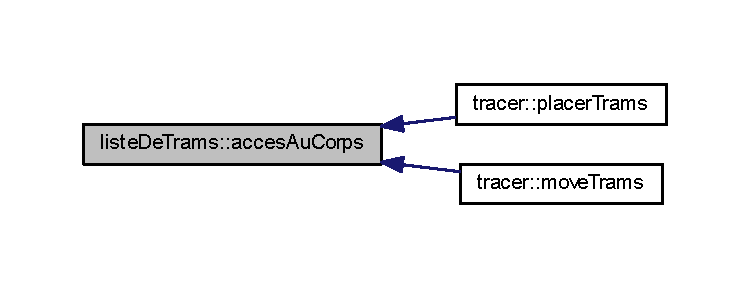
\includegraphics[width=350pt]{classliste_de_trams_a2e66b663287f770c709c16d89424818e_icgraph}
\end{center}
\end{figure}


\index{liste\+De\+Trams@{liste\+De\+Trams}!acces\+Au\+Queue@{acces\+Au\+Queue}}
\index{acces\+Au\+Queue@{acces\+Au\+Queue}!liste\+De\+Trams@{liste\+De\+Trams}}
\subsubsection[{\texorpdfstring{acces\+Au\+Queue() const }{accesAuQueue() const }}]{\setlength{\rightskip}{0pt plus 5cm}{\bf tramway} $\ast$ liste\+De\+Trams\+::acces\+Au\+Queue (
\begin{DoxyParamCaption}
{}
\end{DoxyParamCaption}
) const}\hypertarget{classliste_de_trams_a442cc0dc48c4d8abfd3e8de30a85e24c}{}\label{classliste_de_trams_a442cc0dc48c4d8abfd3e8de30a85e24c}
\begin{DoxyReturn}{Returns}
-\/ le dernier tram de la liste 
\end{DoxyReturn}
\index{liste\+De\+Trams@{liste\+De\+Trams}!acces\+En\+Tete@{acces\+En\+Tete}}
\index{acces\+En\+Tete@{acces\+En\+Tete}!liste\+De\+Trams@{liste\+De\+Trams}}
\subsubsection[{\texorpdfstring{acces\+En\+Tete() const }{accesEnTete() const }}]{\setlength{\rightskip}{0pt plus 5cm}{\bf tramway} $\ast$ liste\+De\+Trams\+::acces\+En\+Tete (
\begin{DoxyParamCaption}
{}
\end{DoxyParamCaption}
) const}\hypertarget{classliste_de_trams_aa494f9ab59eb0250608782b536f2aa5f}{}\label{classliste_de_trams_aa494f9ab59eb0250608782b536f2aa5f}


A\+C\+C\+ES. 

\begin{DoxyReturn}{Returns}
-\/ le premier tram de la liste 
\end{DoxyReturn}
\index{liste\+De\+Trams@{liste\+De\+Trams}!afficher\+Liste@{afficher\+Liste}}
\index{afficher\+Liste@{afficher\+Liste}!liste\+De\+Trams@{liste\+De\+Trams}}
\subsubsection[{\texorpdfstring{afficher\+Liste() const }{afficherListe() const }}]{\setlength{\rightskip}{0pt plus 5cm}void liste\+De\+Trams\+::afficher\+Liste (
\begin{DoxyParamCaption}
{}
\end{DoxyParamCaption}
) const}\hypertarget{classliste_de_trams_ab1d9638e4f071077f5182413ae8b1c8c}{}\label{classliste_de_trams_ab1d9638e4f071077f5182413ae8b1c8c}
Affiche la liste tram au niveau console \index{liste\+De\+Trams@{liste\+De\+Trams}!ajout\+Au\+Corps@{ajout\+Au\+Corps}}
\index{ajout\+Au\+Corps@{ajout\+Au\+Corps}!liste\+De\+Trams@{liste\+De\+Trams}}
\subsubsection[{\texorpdfstring{ajout\+Au\+Corps(int numero, int vitesse\+Max, bool sens, double pos\+X, double pos\+Y, ligne $\ast$ligne\+Affect, int corps)}{ajoutAuCorps(int numero, int vitesseMax, bool sens, double posX, double posY, ligne *ligneAffect, int corps)}}]{\setlength{\rightskip}{0pt plus 5cm}void liste\+De\+Trams\+::ajout\+Au\+Corps (
\begin{DoxyParamCaption}
\item[{int}]{numero, }
\item[{int}]{vitesse\+Max, }
\item[{bool}]{sens, }
\item[{double}]{posX, }
\item[{double}]{posY, }
\item[{{\bf ligne} $\ast$}]{ligne\+Affect, }
\item[{int}]{corps}
\end{DoxyParamCaption}
)}\hypertarget{classliste_de_trams_aae576aa98d9709644fee9dda66ea54f7}{}\label{classliste_de_trams_aae576aa98d9709644fee9dda66ea54f7}

\begin{DoxyParams}[1]{Parameters}
\mbox{\tt in}  & {\em num\+Ligne} & -\/ \\
\hline
\mbox{\tt in}  & {\em vitesse\+Max} & -\/ \\
\hline
\mbox{\tt in}  & {\em sens} & -\/ \\
\hline
\mbox{\tt in}  & {\em posX} & -\/ \\
\hline
\mbox{\tt in}  & {\em posY} & -\/ \\
\hline
\mbox{\tt in}  & {\em corps} & -\/ \\
\hline
\mbox{\tt in}  & {\em ligne\+Affect} & -\/ \\
\hline
\end{DoxyParams}


Here is the call graph for this function\+:
\nopagebreak
\begin{figure}[H]
\begin{center}
\leavevmode
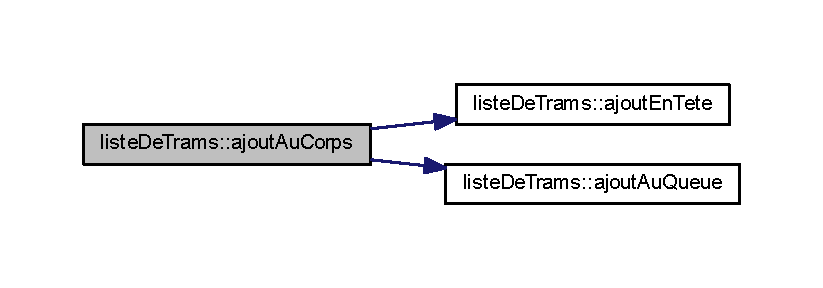
\includegraphics[width=350pt]{classliste_de_trams_aae576aa98d9709644fee9dda66ea54f7_cgraph}
\end{center}
\end{figure}


\index{liste\+De\+Trams@{liste\+De\+Trams}!ajout\+Au\+Queue@{ajout\+Au\+Queue}}
\index{ajout\+Au\+Queue@{ajout\+Au\+Queue}!liste\+De\+Trams@{liste\+De\+Trams}}
\subsubsection[{\texorpdfstring{ajout\+Au\+Queue(int numero, int vitesse\+Max, bool sens, double pos\+X, double pos\+Y, ligne $\ast$ligne\+Affect)}{ajoutAuQueue(int numero, int vitesseMax, bool sens, double posX, double posY, ligne *ligneAffect)}}]{\setlength{\rightskip}{0pt plus 5cm}void liste\+De\+Trams\+::ajout\+Au\+Queue (
\begin{DoxyParamCaption}
\item[{int}]{numero, }
\item[{int}]{vitesse\+Max, }
\item[{bool}]{sens, }
\item[{double}]{posX, }
\item[{double}]{posY, }
\item[{{\bf ligne} $\ast$}]{ligne\+Affect}
\end{DoxyParamCaption}
)}\hypertarget{classliste_de_trams_af969635f70bda1d3b429a1220e649d7c}{}\label{classliste_de_trams_af969635f70bda1d3b429a1220e649d7c}

\begin{DoxyParams}[1]{Parameters}
\mbox{\tt in}  & {\em num\+Ligne} & -\/ \\
\hline
\mbox{\tt in}  & {\em vitesse\+Max} & -\/ \\
\hline
\mbox{\tt in}  & {\em sens} & -\/ \\
\hline
\mbox{\tt in}  & {\em posX} & -\/ \\
\hline
\mbox{\tt in}  & {\em posY} & -\/ \\
\hline
\mbox{\tt in}  & {\em ligne\+Affect} & -\/ \\
\hline
\end{DoxyParams}


Here is the caller graph for this function\+:
\nopagebreak
\begin{figure}[H]
\begin{center}
\leavevmode
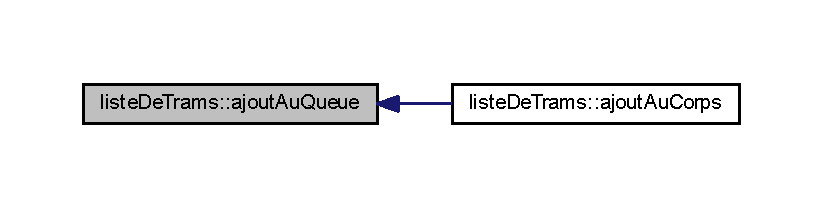
\includegraphics[width=350pt]{classliste_de_trams_af969635f70bda1d3b429a1220e649d7c_icgraph}
\end{center}
\end{figure}


\index{liste\+De\+Trams@{liste\+De\+Trams}!ajout\+En\+Tete@{ajout\+En\+Tete}}
\index{ajout\+En\+Tete@{ajout\+En\+Tete}!liste\+De\+Trams@{liste\+De\+Trams}}
\subsubsection[{\texorpdfstring{ajout\+En\+Tete(int numero, int vitesse\+Max, bool sens, double pos\+X, double pos\+Y, ligne $\ast$ligne\+Affect)}{ajoutEnTete(int numero, int vitesseMax, bool sens, double posX, double posY, ligne *ligneAffect)}}]{\setlength{\rightskip}{0pt plus 5cm}void liste\+De\+Trams\+::ajout\+En\+Tete (
\begin{DoxyParamCaption}
\item[{int}]{num\+Ligne, }
\item[{int}]{vitesse\+Max, }
\item[{bool}]{sens, }
\item[{double}]{posX, }
\item[{double}]{posY, }
\item[{{\bf ligne} $\ast$}]{ligne\+Affect}
\end{DoxyParamCaption}
)}\hypertarget{classliste_de_trams_acc9f9a3e125a1801cfe108a4a9b27cfc}{}\label{classliste_de_trams_acc9f9a3e125a1801cfe108a4a9b27cfc}


A\+J\+O\+U\+TS. 


\begin{DoxyParams}[1]{Parameters}
\mbox{\tt in}  & {\em num\+Ligne} & -\/ \\
\hline
\mbox{\tt in}  & {\em vitesse\+Max} & -\/ \\
\hline
\mbox{\tt in}  & {\em sens} & -\/ \\
\hline
\mbox{\tt in}  & {\em posX} & -\/ \\
\hline
\mbox{\tt in}  & {\em posY} & -\/ \\
\hline
\mbox{\tt in}  & {\em ligne\+Affect} & -\/ \\
\hline
\end{DoxyParams}


Here is the caller graph for this function\+:
\nopagebreak
\begin{figure}[H]
\begin{center}
\leavevmode
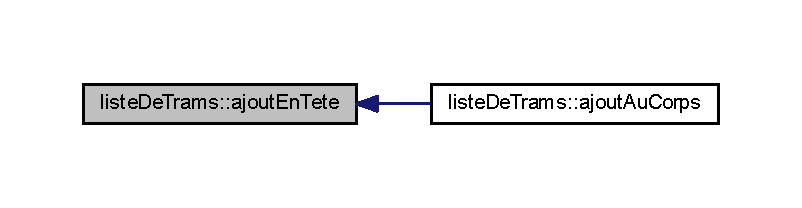
\includegraphics[width=350pt]{classliste_de_trams_acc9f9a3e125a1801cfe108a4a9b27cfc_icgraph}
\end{center}
\end{figure}


\index{liste\+De\+Trams@{liste\+De\+Trams}!est\+Vide@{est\+Vide}}
\index{est\+Vide@{est\+Vide}!liste\+De\+Trams@{liste\+De\+Trams}}
\subsubsection[{\texorpdfstring{est\+Vide() const }{estVide() const }}]{\setlength{\rightskip}{0pt plus 5cm}bool liste\+De\+Trams\+::est\+Vide (
\begin{DoxyParamCaption}
{}
\end{DoxyParamCaption}
) const}\hypertarget{classliste_de_trams_a137520c68e8c14b3cbfa1711d21849a1}{}\label{classliste_de_trams_a137520c68e8c14b3cbfa1711d21849a1}
\begin{DoxyReturn}{Returns}
-\/ si le nombre tram =0 
\end{DoxyReturn}
\index{liste\+De\+Trams@{liste\+De\+Trams}!nombre\+De\+Trams@{nombre\+De\+Trams}}
\index{nombre\+De\+Trams@{nombre\+De\+Trams}!liste\+De\+Trams@{liste\+De\+Trams}}
\subsubsection[{\texorpdfstring{nombre\+De\+Trams() const }{nombreDeTrams() const }}]{\setlength{\rightskip}{0pt plus 5cm}int liste\+De\+Trams\+::nombre\+De\+Trams (
\begin{DoxyParamCaption}
{}
\end{DoxyParamCaption}
) const}\hypertarget{classliste_de_trams_afd3b9e87aa935dca81ce3f6d1aea6f75}{}\label{classliste_de_trams_afd3b9e87aa935dca81ce3f6d1aea6f75}
\begin{DoxyReturn}{Returns}
-\/ le nombre tram 
\end{DoxyReturn}


Here is the caller graph for this function\+:
\nopagebreak
\begin{figure}[H]
\begin{center}
\leavevmode
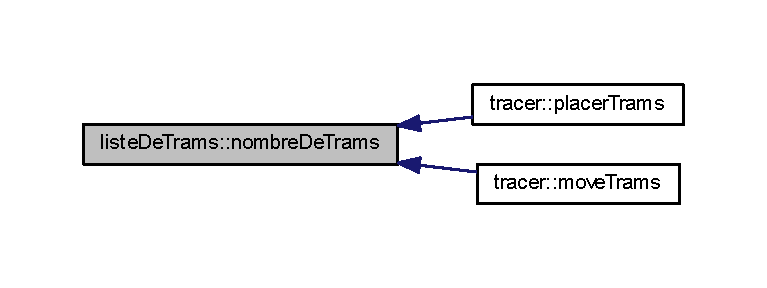
\includegraphics[width=350pt]{classliste_de_trams_afd3b9e87aa935dca81ce3f6d1aea6f75_icgraph}
\end{center}
\end{figure}


\index{liste\+De\+Trams@{liste\+De\+Trams}!suppr\+Au\+Corps@{suppr\+Au\+Corps}}
\index{suppr\+Au\+Corps@{suppr\+Au\+Corps}!liste\+De\+Trams@{liste\+De\+Trams}}
\subsubsection[{\texorpdfstring{suppr\+Au\+Corps(int corps)}{supprAuCorps(int corps)}}]{\setlength{\rightskip}{0pt plus 5cm}void liste\+De\+Trams\+::suppr\+Au\+Corps (
\begin{DoxyParamCaption}
\item[{int}]{corps}
\end{DoxyParamCaption}
)}\hypertarget{classliste_de_trams_a718310361597fbe63375c37f3028defa}{}\label{classliste_de_trams_a718310361597fbe63375c37f3028defa}
delete a une position int corps 

Here is the call graph for this function\+:
\nopagebreak
\begin{figure}[H]
\begin{center}
\leavevmode
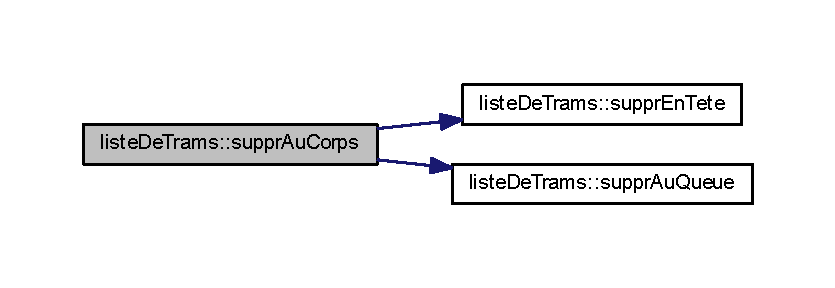
\includegraphics[width=350pt]{classliste_de_trams_a718310361597fbe63375c37f3028defa_cgraph}
\end{center}
\end{figure}


\index{liste\+De\+Trams@{liste\+De\+Trams}!suppr\+Au\+Queue@{suppr\+Au\+Queue}}
\index{suppr\+Au\+Queue@{suppr\+Au\+Queue}!liste\+De\+Trams@{liste\+De\+Trams}}
\subsubsection[{\texorpdfstring{suppr\+Au\+Queue()}{supprAuQueue()}}]{\setlength{\rightskip}{0pt plus 5cm}void liste\+De\+Trams\+::suppr\+Au\+Queue (
\begin{DoxyParamCaption}
{}
\end{DoxyParamCaption}
)}\hypertarget{classliste_de_trams_aea83e66431a0a5ff31a631a04f3284cc}{}\label{classliste_de_trams_aea83e66431a0a5ff31a631a04f3284cc}
delete au queue 

Here is the caller graph for this function\+:
\nopagebreak
\begin{figure}[H]
\begin{center}
\leavevmode
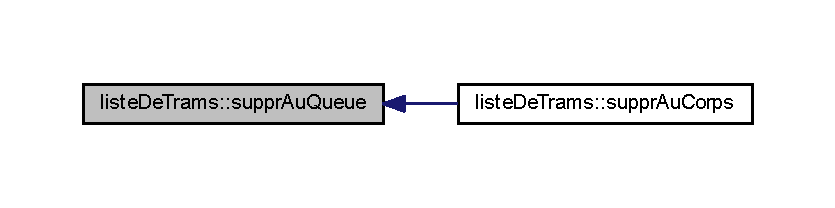
\includegraphics[width=350pt]{classliste_de_trams_aea83e66431a0a5ff31a631a04f3284cc_icgraph}
\end{center}
\end{figure}


\index{liste\+De\+Trams@{liste\+De\+Trams}!suppr\+En\+Tete@{suppr\+En\+Tete}}
\index{suppr\+En\+Tete@{suppr\+En\+Tete}!liste\+De\+Trams@{liste\+De\+Trams}}
\subsubsection[{\texorpdfstring{suppr\+En\+Tete()}{supprEnTete()}}]{\setlength{\rightskip}{0pt plus 5cm}void liste\+De\+Trams\+::suppr\+En\+Tete (
\begin{DoxyParamCaption}
{}
\end{DoxyParamCaption}
)}\hypertarget{classliste_de_trams_a495cc9d541621a18e3c10817e62d31bd}{}\label{classliste_de_trams_a495cc9d541621a18e3c10817e62d31bd}


S\+U\+P\+P\+R\+E\+S\+S\+I\+O\+NS. 

delete en tete 

Here is the caller graph for this function\+:
\nopagebreak
\begin{figure}[H]
\begin{center}
\leavevmode
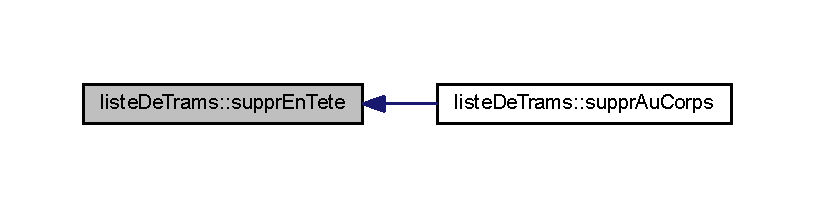
\includegraphics[width=350pt]{classliste_de_trams_a495cc9d541621a18e3c10817e62d31bd_icgraph}
\end{center}
\end{figure}




The documentation for this class was generated from the following files\+:\begin{DoxyCompactItemize}
\item 
C\+:/\+Users/oumar12/\+Desktop/\+T\+R\+A\+M\+W\+A\+Y\+S/\+T\+R\+A\+M\+W\+A\+Y\+S/\hyperlink{liste_de_tramway_8h}{liste\+De\+Tramway.\+h}\item 
C\+:/\+Users/oumar12/\+Desktop/\+T\+R\+A\+M\+W\+A\+Y\+S/\+T\+R\+A\+M\+W\+A\+Y\+S/\hyperlink{liste_de_tramway_8cpp}{liste\+De\+Tramway.\+cpp}\end{DoxyCompactItemize}

\hypertarget{classtracer}{}\section{tracer Class Reference}
\label{classtracer}\index{tracer@{tracer}}


{\ttfamily \#include $<$tracer.\+h$>$}

\subsection*{Public Member Functions}
\begin{DoxyCompactItemize}
\item 
\hyperlink{classtracer_ad341e6024da0488dd9c3ff9767333ab0}{tracer} (int largeur, int hauteur)
\item 
void \hyperlink{classtracer_a4d68d6842a65f6f153026357847b49fc}{placer\+Arret} (\hyperlink{classarret}{arret} $\ast$un\+Arret) const 
\item 
void \hyperlink{classtracer_a9d82959867464033e3b68892023969ce}{placer\+Arrets} (\hyperlink{classligne}{ligne} $\ast$une\+Ligne) const 
\item 
void \hyperlink{classtracer_a37ba471b0824655b4a6a2820d6b7ee56}{liens\+Arrets} (\hyperlink{classligne}{ligne} $\ast$une\+Ligne) const 
\item 
void \hyperlink{classtracer_a747a35b63db6765185c0de6f652f8c13}{placer\+Tram} (\hyperlink{classtramway}{tramway} $\ast$tram) const 
\item 
void \hyperlink{classtracer_ae50f04257d21db5b947cd8548414a0f7}{placer\+Trams} (\hyperlink{classligne}{ligne} $\ast$une\+Ligne) const 
\item 
void \hyperlink{classtracer_a31536796cd89d2ee47a7d5e17432bc65}{build\+Ligne} (\hyperlink{classligne}{ligne} $\ast$une\+Ligne) const 
\item 
void \hyperlink{classtracer_a59f9f4e714b1ebcf114ae7ca648e7d8c}{move\+Tram} (\hyperlink{classtramway}{tramway} $\ast$tram)
\item 
void \hyperlink{classtracer_a206500c8582dbad012b898dc922fc5a7}{move\+Trams} (\hyperlink{classligne}{ligne} $\ast$une\+Ligne)
\item 
void \hyperlink{classtracer_a1ac543894333a48a09a1a423d33b20a5}{simuler\+Tram} (std\+::vector$<$ \hyperlink{classligne}{ligne} $\ast$ $>$ \&lignes, int temps\+Simul)
\end{DoxyCompactItemize}


\subsection{Constructor \& Destructor Documentation}
\index{tracer@{tracer}!tracer@{tracer}}
\index{tracer@{tracer}!tracer@{tracer}}
\subsubsection[{\texorpdfstring{tracer(int largeur, int hauteur)}{tracer(int largeur, int hauteur)}}]{\setlength{\rightskip}{0pt plus 5cm}tracer\+::tracer (
\begin{DoxyParamCaption}
\item[{int}]{largeur, }
\item[{int}]{hauteur}
\end{DoxyParamCaption}
)}\hypertarget{classtracer_ad341e6024da0488dd9c3ff9767333ab0}{}\label{classtracer_ad341e6024da0488dd9c3ff9767333ab0}


\subsection{Member Function Documentation}
\index{tracer@{tracer}!build\+Ligne@{build\+Ligne}}
\index{build\+Ligne@{build\+Ligne}!tracer@{tracer}}
\subsubsection[{\texorpdfstring{build\+Ligne(ligne $\ast$une\+Ligne) const }{buildLigne(ligne *uneLigne) const }}]{\setlength{\rightskip}{0pt plus 5cm}void tracer\+::build\+Ligne (
\begin{DoxyParamCaption}
\item[{{\bf ligne} $\ast$}]{une\+Ligne}
\end{DoxyParamCaption}
) const}\hypertarget{classtracer_a31536796cd89d2ee47a7d5e17432bc65}{}\label{classtracer_a31536796cd89d2ee47a7d5e17432bc65}
\index{tracer@{tracer}!liens\+Arrets@{liens\+Arrets}}
\index{liens\+Arrets@{liens\+Arrets}!tracer@{tracer}}
\subsubsection[{\texorpdfstring{liens\+Arrets(ligne $\ast$une\+Ligne) const }{liensArrets(ligne *uneLigne) const }}]{\setlength{\rightskip}{0pt plus 5cm}void tracer\+::liens\+Arrets (
\begin{DoxyParamCaption}
\item[{{\bf ligne} $\ast$}]{une\+Ligne}
\end{DoxyParamCaption}
) const}\hypertarget{classtracer_a37ba471b0824655b4a6a2820d6b7ee56}{}\label{classtracer_a37ba471b0824655b4a6a2820d6b7ee56}


Here is the call graph for this function\+:
\nopagebreak
\begin{figure}[H]
\begin{center}
\leavevmode
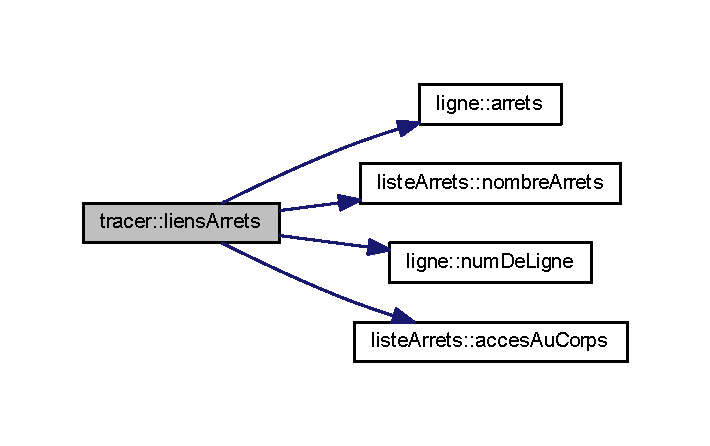
\includegraphics[width=341pt]{classtracer_a37ba471b0824655b4a6a2820d6b7ee56_cgraph}
\end{center}
\end{figure}


\index{tracer@{tracer}!move\+Tram@{move\+Tram}}
\index{move\+Tram@{move\+Tram}!tracer@{tracer}}
\subsubsection[{\texorpdfstring{move\+Tram(tramway $\ast$tram)}{moveTram(tramway *tram)}}]{\setlength{\rightskip}{0pt plus 5cm}void tracer\+::move\+Tram (
\begin{DoxyParamCaption}
\item[{{\bf tramway} $\ast$}]{tram}
\end{DoxyParamCaption}
)}\hypertarget{classtracer_a59f9f4e714b1ebcf114ae7ca648e7d8c}{}\label{classtracer_a59f9f4e714b1ebcf114ae7ca648e7d8c}


Here is the call graph for this function\+:
\nopagebreak
\begin{figure}[H]
\begin{center}
\leavevmode
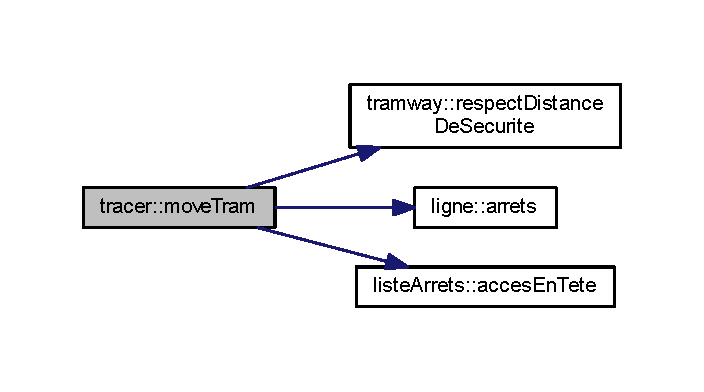
\includegraphics[width=338pt]{classtracer_a59f9f4e714b1ebcf114ae7ca648e7d8c_cgraph}
\end{center}
\end{figure}


\index{tracer@{tracer}!move\+Trams@{move\+Trams}}
\index{move\+Trams@{move\+Trams}!tracer@{tracer}}
\subsubsection[{\texorpdfstring{move\+Trams(ligne $\ast$une\+Ligne)}{moveTrams(ligne *uneLigne)}}]{\setlength{\rightskip}{0pt plus 5cm}void tracer\+::move\+Trams (
\begin{DoxyParamCaption}
\item[{{\bf ligne} $\ast$}]{une\+Ligne}
\end{DoxyParamCaption}
)}\hypertarget{classtracer_a206500c8582dbad012b898dc922fc5a7}{}\label{classtracer_a206500c8582dbad012b898dc922fc5a7}


Here is the call graph for this function\+:
\nopagebreak
\begin{figure}[H]
\begin{center}
\leavevmode
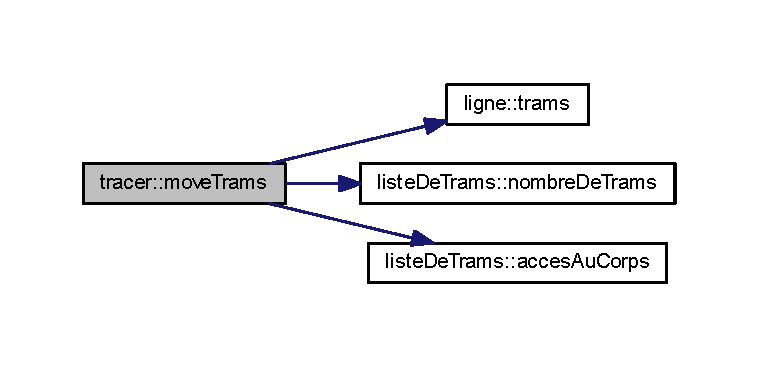
\includegraphics[width=350pt]{classtracer_a206500c8582dbad012b898dc922fc5a7_cgraph}
\end{center}
\end{figure}


\index{tracer@{tracer}!placer\+Arret@{placer\+Arret}}
\index{placer\+Arret@{placer\+Arret}!tracer@{tracer}}
\subsubsection[{\texorpdfstring{placer\+Arret(arret $\ast$un\+Arret) const }{placerArret(arret *unArret) const }}]{\setlength{\rightskip}{0pt plus 5cm}void tracer\+::placer\+Arret (
\begin{DoxyParamCaption}
\item[{{\bf arret} $\ast$}]{un\+Arret}
\end{DoxyParamCaption}
) const}\hypertarget{classtracer_a4d68d6842a65f6f153026357847b49fc}{}\label{classtracer_a4d68d6842a65f6f153026357847b49fc}
\index{tracer@{tracer}!placer\+Arrets@{placer\+Arrets}}
\index{placer\+Arrets@{placer\+Arrets}!tracer@{tracer}}
\subsubsection[{\texorpdfstring{placer\+Arrets(ligne $\ast$une\+Ligne) const }{placerArrets(ligne *uneLigne) const }}]{\setlength{\rightskip}{0pt plus 5cm}void tracer\+::placer\+Arrets (
\begin{DoxyParamCaption}
\item[{{\bf ligne} $\ast$}]{une\+Ligne}
\end{DoxyParamCaption}
) const}\hypertarget{classtracer_a9d82959867464033e3b68892023969ce}{}\label{classtracer_a9d82959867464033e3b68892023969ce}


Here is the call graph for this function\+:
\nopagebreak
\begin{figure}[H]
\begin{center}
\leavevmode
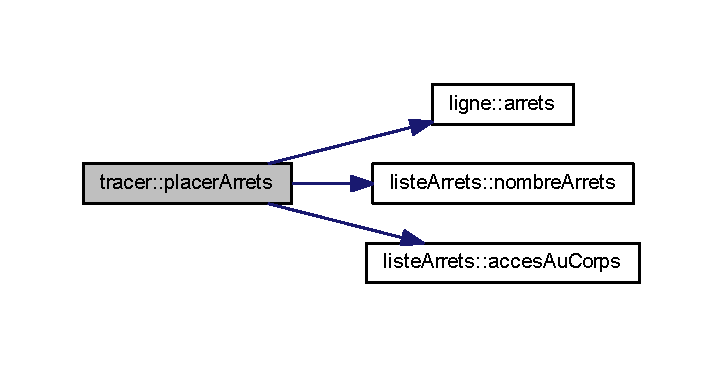
\includegraphics[width=347pt]{classtracer_a9d82959867464033e3b68892023969ce_cgraph}
\end{center}
\end{figure}


\index{tracer@{tracer}!placer\+Tram@{placer\+Tram}}
\index{placer\+Tram@{placer\+Tram}!tracer@{tracer}}
\subsubsection[{\texorpdfstring{placer\+Tram(tramway $\ast$tram) const }{placerTram(tramway *tram) const }}]{\setlength{\rightskip}{0pt plus 5cm}void tracer\+::placer\+Tram (
\begin{DoxyParamCaption}
\item[{{\bf tramway} $\ast$}]{tram}
\end{DoxyParamCaption}
) const}\hypertarget{classtracer_a747a35b63db6765185c0de6f652f8c13}{}\label{classtracer_a747a35b63db6765185c0de6f652f8c13}
\index{tracer@{tracer}!placer\+Trams@{placer\+Trams}}
\index{placer\+Trams@{placer\+Trams}!tracer@{tracer}}
\subsubsection[{\texorpdfstring{placer\+Trams(ligne $\ast$une\+Ligne) const }{placerTrams(ligne *uneLigne) const }}]{\setlength{\rightskip}{0pt plus 5cm}void tracer\+::placer\+Trams (
\begin{DoxyParamCaption}
\item[{{\bf ligne} $\ast$}]{une\+Ligne}
\end{DoxyParamCaption}
) const}\hypertarget{classtracer_ae50f04257d21db5b947cd8548414a0f7}{}\label{classtracer_ae50f04257d21db5b947cd8548414a0f7}


Here is the call graph for this function\+:
\nopagebreak
\begin{figure}[H]
\begin{center}
\leavevmode
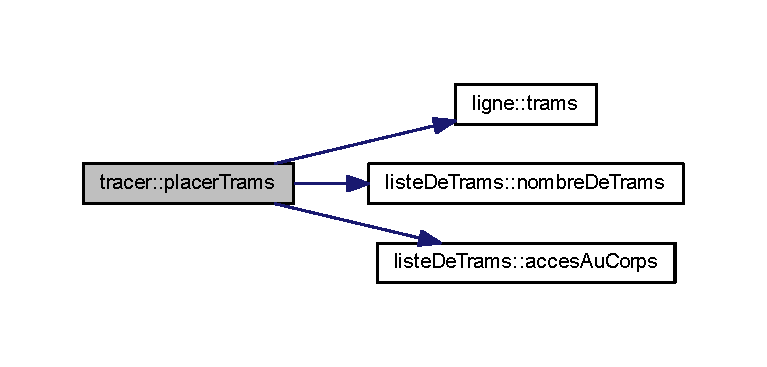
\includegraphics[width=350pt]{classtracer_ae50f04257d21db5b947cd8548414a0f7_cgraph}
\end{center}
\end{figure}


\index{tracer@{tracer}!simuler\+Tram@{simuler\+Tram}}
\index{simuler\+Tram@{simuler\+Tram}!tracer@{tracer}}
\subsubsection[{\texorpdfstring{simuler\+Tram(std\+::vector$<$ ligne $\ast$ $>$ \&lignes, int temps\+Simul)}{simulerTram(std::vector< ligne * > &lignes, int tempsSimul)}}]{\setlength{\rightskip}{0pt plus 5cm}void tracer\+::simuler\+Tram (
\begin{DoxyParamCaption}
\item[{std\+::vector$<$ {\bf ligne} $\ast$ $>$ \&}]{lignes, }
\item[{int}]{temps\+Simul}
\end{DoxyParamCaption}
)}\hypertarget{classtracer_a1ac543894333a48a09a1a423d33b20a5}{}\label{classtracer_a1ac543894333a48a09a1a423d33b20a5}


Here is the caller graph for this function\+:
\nopagebreak
\begin{figure}[H]
\begin{center}
\leavevmode
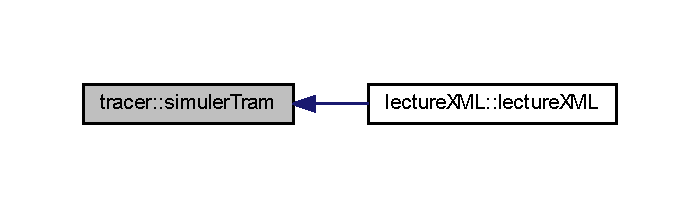
\includegraphics[width=336pt]{classtracer_a1ac543894333a48a09a1a423d33b20a5_icgraph}
\end{center}
\end{figure}




The documentation for this class was generated from the following files\+:\begin{DoxyCompactItemize}
\item 
C\+:/\+Users/oumar12/\+Desktop/\+T\+R\+A\+M\+W\+A\+Y\+S/\+T\+R\+A\+M\+W\+A\+Y\+S/\hyperlink{tracer_8h}{tracer.\+h}\item 
C\+:/\+Users/oumar12/\+Desktop/\+T\+R\+A\+M\+W\+A\+Y\+S/\+T\+R\+A\+M\+W\+A\+Y\+S/\hyperlink{tracer_8cpp}{tracer.\+cpp}\end{DoxyCompactItemize}

\hypertarget{classtramway}{}\section{tramway Class Reference}
\label{classtramway}\index{tramway@{tramway}}


{\ttfamily \#include $<$liste\+De\+Tramway.\+h$>$}



Collaboration diagram for tramway\+:
\nopagebreak
\begin{figure}[H]
\begin{center}
\leavevmode
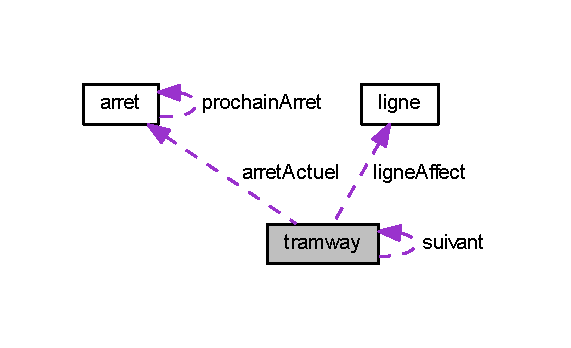
\includegraphics[width=274pt]{classtramway__coll__graph}
\end{center}
\end{figure}
\subsection*{Public Member Functions}
\begin{DoxyCompactItemize}
\item 
\hyperlink{classtramway_a3f1e91b979ea3309cd93208439fb5a10}{tramway} (int \hyperlink{classtramway_a937d549fcbdbe222ea08e4ec085bb19b}{num\+Ligne}, int \hyperlink{classtramway_a401f568b9c8cedcf0c359eb68ea8865d}{vitesse\+Max}, bool \hyperlink{classtramway_abc99be632a1ef40a7eae8bb46ac364f6}{sens}, double \hyperlink{classtramway_a0ba5b158240fe160ee8b91c74b4010f5}{posX}, double \hyperlink{classtramway_afb1214281e7e1b2c9a9fd9a5d322e836}{posY}, \hyperlink{classligne}{ligne} $\ast$\hyperlink{classtramway_a0506569903981a08b8835a73fc49609b}{ligne\+Affect})
\item 
bool \hyperlink{classtramway_ac11a2d8761217b5db1253cc35ea67a66}{respect\+Distance\+De\+Securite} ()
\end{DoxyCompactItemize}
\subsection*{Public Attributes}
\begin{DoxyCompactItemize}
\item 
int \hyperlink{classtramway_a937d549fcbdbe222ea08e4ec085bb19b}{num\+Ligne}
\item 
int \hyperlink{classtramway_a401f568b9c8cedcf0c359eb68ea8865d}{vitesse\+Max}
\item 
bool \hyperlink{classtramway_abc99be632a1ef40a7eae8bb46ac364f6}{sens}
\item 
double \hyperlink{classtramway_a0ba5b158240fe160ee8b91c74b4010f5}{posX}
\item 
double \hyperlink{classtramway_afb1214281e7e1b2c9a9fd9a5d322e836}{posY}
\item 
\hyperlink{classligne}{ligne} $\ast$ \hyperlink{classtramway_a0506569903981a08b8835a73fc49609b}{ligne\+Affect}
\item 
\hyperlink{classtramway}{tramway} $\ast$ \hyperlink{classtramway_a1ed327c50d74d61632664f0f460c6cf2}{suivant}
\item 
\hyperlink{classarret}{arret} $\ast$ \hyperlink{classtramway_a316032ab458b4ccf96b3f3f1bf327ee2}{arret\+Actuel}
\item 
int \hyperlink{classtramway_a59e30ad7e6df61e54fe2b326bd9e6134}{distance\+Securite}
\item 
int \hyperlink{classtramway_a85b44399cbbf04ec765d114465a4aa1f}{distance\+Arret}
\item 
int \hyperlink{classtramway_a5eab187ab73b4b91a158dc05fd8ed066}{vitesse\+Actuelle}
\item 
bool \hyperlink{classtramway_acfb0a0666823107c15ac26f074a67d79}{terminus}
\end{DoxyCompactItemize}
\subsection*{Friends}
\begin{DoxyCompactItemize}
\item 
class \hyperlink{classtramway_a769de17fc42804fb0d2a6751abb27e2f}{liste\+De\+Trams}
\end{DoxyCompactItemize}


\subsection{Constructor \& Destructor Documentation}
\index{tramway@{tramway}!tramway@{tramway}}
\index{tramway@{tramway}!tramway@{tramway}}
\subsubsection[{\texorpdfstring{tramway(int num\+Ligne, int vitesse\+Max, bool sens, double pos\+X, double pos\+Y, ligne $\ast$ligne\+Affect)}{tramway(int numLigne, int vitesseMax, bool sens, double posX, double posY, ligne *ligneAffect)}}]{\setlength{\rightskip}{0pt plus 5cm}tramway\+::tramway (
\begin{DoxyParamCaption}
\item[{int}]{num\+Ligne, }
\item[{int}]{vitesse\+Max, }
\item[{bool}]{sens, }
\item[{double}]{posX, }
\item[{double}]{posY, }
\item[{{\bf ligne} $\ast$}]{ligne\+Affect}
\end{DoxyParamCaption}
)}\hypertarget{classtramway_a3f1e91b979ea3309cd93208439fb5a10}{}\label{classtramway_a3f1e91b979ea3309cd93208439fb5a10}
Constructeur tramway 
\begin{DoxyParams}[1]{Parameters}
\mbox{\tt in}  & {\em num\+Ligne} & -\/ \\
\hline
\mbox{\tt in}  & {\em vitesse\+Max} & -\/ \\
\hline
\mbox{\tt in}  & {\em sens} & -\/ \\
\hline
\mbox{\tt in}  & {\em posX} & -\/ \\
\hline
\mbox{\tt in}  & {\em posY} & -\/ \\
\hline
\mbox{\tt in}  & {\em ligne\+Affect} & -\/ \\
\hline
\end{DoxyParams}


\subsection{Member Function Documentation}
\index{tramway@{tramway}!respect\+Distance\+De\+Securite@{respect\+Distance\+De\+Securite}}
\index{respect\+Distance\+De\+Securite@{respect\+Distance\+De\+Securite}!tramway@{tramway}}
\subsubsection[{\texorpdfstring{respect\+Distance\+De\+Securite()}{respectDistanceDeSecurite()}}]{\setlength{\rightskip}{0pt plus 5cm}bool tramway\+::respect\+Distance\+De\+Securite (
\begin{DoxyParamCaption}
{}
\end{DoxyParamCaption}
)}\hypertarget{classtramway_ac11a2d8761217b5db1253cc35ea67a66}{}\label{classtramway_ac11a2d8761217b5db1253cc35ea67a66}
\begin{DoxyReturn}{Returns}
-\/ si la distance est respectee 
\end{DoxyReturn}


Here is the caller graph for this function\+:
\nopagebreak
\begin{figure}[H]
\begin{center}
\leavevmode
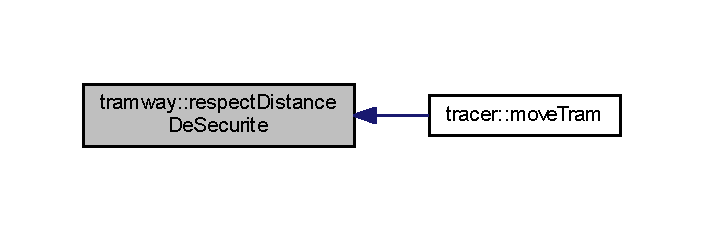
\includegraphics[width=338pt]{classtramway_ac11a2d8761217b5db1253cc35ea67a66_icgraph}
\end{center}
\end{figure}




\subsection{Friends And Related Function Documentation}
\index{tramway@{tramway}!liste\+De\+Trams@{liste\+De\+Trams}}
\index{liste\+De\+Trams@{liste\+De\+Trams}!tramway@{tramway}}
\subsubsection[{\texorpdfstring{liste\+De\+Trams}{listeDeTrams}}]{\setlength{\rightskip}{0pt plus 5cm}friend class {\bf liste\+De\+Trams}\hspace{0.3cm}{\ttfamily [friend]}}\hypertarget{classtramway_a769de17fc42804fb0d2a6751abb27e2f}{}\label{classtramway_a769de17fc42804fb0d2a6751abb27e2f}


\subsection{Member Data Documentation}
\index{tramway@{tramway}!arret\+Actuel@{arret\+Actuel}}
\index{arret\+Actuel@{arret\+Actuel}!tramway@{tramway}}
\subsubsection[{\texorpdfstring{arret\+Actuel}{arretActuel}}]{\setlength{\rightskip}{0pt plus 5cm}{\bf arret}$\ast$ tramway\+::arret\+Actuel}\hypertarget{classtramway_a316032ab458b4ccf96b3f3f1bf327ee2}{}\label{classtramway_a316032ab458b4ccf96b3f3f1bf327ee2}
\index{tramway@{tramway}!distance\+Arret@{distance\+Arret}}
\index{distance\+Arret@{distance\+Arret}!tramway@{tramway}}
\subsubsection[{\texorpdfstring{distance\+Arret}{distanceArret}}]{\setlength{\rightskip}{0pt plus 5cm}int tramway\+::distance\+Arret}\hypertarget{classtramway_a85b44399cbbf04ec765d114465a4aa1f}{}\label{classtramway_a85b44399cbbf04ec765d114465a4aa1f}
\index{tramway@{tramway}!distance\+Securite@{distance\+Securite}}
\index{distance\+Securite@{distance\+Securite}!tramway@{tramway}}
\subsubsection[{\texorpdfstring{distance\+Securite}{distanceSecurite}}]{\setlength{\rightskip}{0pt plus 5cm}int tramway\+::distance\+Securite}\hypertarget{classtramway_a59e30ad7e6df61e54fe2b326bd9e6134}{}\label{classtramway_a59e30ad7e6df61e54fe2b326bd9e6134}
\index{tramway@{tramway}!ligne\+Affect@{ligne\+Affect}}
\index{ligne\+Affect@{ligne\+Affect}!tramway@{tramway}}
\subsubsection[{\texorpdfstring{ligne\+Affect}{ligneAffect}}]{\setlength{\rightskip}{0pt plus 5cm}{\bf ligne}$\ast$ tramway\+::ligne\+Affect}\hypertarget{classtramway_a0506569903981a08b8835a73fc49609b}{}\label{classtramway_a0506569903981a08b8835a73fc49609b}
\index{tramway@{tramway}!num\+Ligne@{num\+Ligne}}
\index{num\+Ligne@{num\+Ligne}!tramway@{tramway}}
\subsubsection[{\texorpdfstring{num\+Ligne}{numLigne}}]{\setlength{\rightskip}{0pt plus 5cm}int tramway\+::num\+Ligne}\hypertarget{classtramway_a937d549fcbdbe222ea08e4ec085bb19b}{}\label{classtramway_a937d549fcbdbe222ea08e4ec085bb19b}
\index{tramway@{tramway}!posX@{posX}}
\index{posX@{posX}!tramway@{tramway}}
\subsubsection[{\texorpdfstring{posX}{posX}}]{\setlength{\rightskip}{0pt plus 5cm}double tramway\+::posX}\hypertarget{classtramway_a0ba5b158240fe160ee8b91c74b4010f5}{}\label{classtramway_a0ba5b158240fe160ee8b91c74b4010f5}
\index{tramway@{tramway}!posY@{posY}}
\index{posY@{posY}!tramway@{tramway}}
\subsubsection[{\texorpdfstring{posY}{posY}}]{\setlength{\rightskip}{0pt plus 5cm}double tramway\+::posY}\hypertarget{classtramway_afb1214281e7e1b2c9a9fd9a5d322e836}{}\label{classtramway_afb1214281e7e1b2c9a9fd9a5d322e836}
\index{tramway@{tramway}!sens@{sens}}
\index{sens@{sens}!tramway@{tramway}}
\subsubsection[{\texorpdfstring{sens}{sens}}]{\setlength{\rightskip}{0pt plus 5cm}bool tramway\+::sens}\hypertarget{classtramway_abc99be632a1ef40a7eae8bb46ac364f6}{}\label{classtramway_abc99be632a1ef40a7eae8bb46ac364f6}
\index{tramway@{tramway}!suivant@{suivant}}
\index{suivant@{suivant}!tramway@{tramway}}
\subsubsection[{\texorpdfstring{suivant}{suivant}}]{\setlength{\rightskip}{0pt plus 5cm}{\bf tramway}$\ast$ tramway\+::suivant}\hypertarget{classtramway_a1ed327c50d74d61632664f0f460c6cf2}{}\label{classtramway_a1ed327c50d74d61632664f0f460c6cf2}
\index{tramway@{tramway}!terminus@{terminus}}
\index{terminus@{terminus}!tramway@{tramway}}
\subsubsection[{\texorpdfstring{terminus}{terminus}}]{\setlength{\rightskip}{0pt plus 5cm}bool tramway\+::terminus}\hypertarget{classtramway_acfb0a0666823107c15ac26f074a67d79}{}\label{classtramway_acfb0a0666823107c15ac26f074a67d79}
\index{tramway@{tramway}!vitesse\+Actuelle@{vitesse\+Actuelle}}
\index{vitesse\+Actuelle@{vitesse\+Actuelle}!tramway@{tramway}}
\subsubsection[{\texorpdfstring{vitesse\+Actuelle}{vitesseActuelle}}]{\setlength{\rightskip}{0pt plus 5cm}int tramway\+::vitesse\+Actuelle}\hypertarget{classtramway_a5eab187ab73b4b91a158dc05fd8ed066}{}\label{classtramway_a5eab187ab73b4b91a158dc05fd8ed066}
\index{tramway@{tramway}!vitesse\+Max@{vitesse\+Max}}
\index{vitesse\+Max@{vitesse\+Max}!tramway@{tramway}}
\subsubsection[{\texorpdfstring{vitesse\+Max}{vitesseMax}}]{\setlength{\rightskip}{0pt plus 5cm}int tramway\+::vitesse\+Max}\hypertarget{classtramway_a401f568b9c8cedcf0c359eb68ea8865d}{}\label{classtramway_a401f568b9c8cedcf0c359eb68ea8865d}


The documentation for this class was generated from the following files\+:\begin{DoxyCompactItemize}
\item 
C\+:/\+Users/oumar12/\+Desktop/\+T\+R\+A\+M\+W\+A\+Y\+S/\+T\+R\+A\+M\+W\+A\+Y\+S/\hyperlink{liste_de_tramway_8h}{liste\+De\+Tramway.\+h}\item 
C\+:/\+Users/oumar12/\+Desktop/\+T\+R\+A\+M\+W\+A\+Y\+S/\+T\+R\+A\+M\+W\+A\+Y\+S/\hyperlink{liste_de_tramway_8cpp}{liste\+De\+Tramway.\+cpp}\end{DoxyCompactItemize}

\chapter{File Documentation}
\hypertarget{lecture_x_m_l_8cpp}{}\section{C\+:/\+Users/oumar12/\+Desktop/\+T\+R\+A\+M\+W\+A\+Y\+S/\+T\+R\+A\+M\+W\+A\+Y\+S/lecture\+X\+ML.cpp File Reference}
\label{lecture_x_m_l_8cpp}\index{C\+:/\+Users/oumar12/\+Desktop/\+T\+R\+A\+M\+W\+A\+Y\+S/\+T\+R\+A\+M\+W\+A\+Y\+S/lecture\+X\+M\+L.\+cpp@{C\+:/\+Users/oumar12/\+Desktop/\+T\+R\+A\+M\+W\+A\+Y\+S/\+T\+R\+A\+M\+W\+A\+Y\+S/lecture\+X\+M\+L.\+cpp}}
{\ttfamily \#include \char`\"{}liste\+De\+Tramway.\+h\char`\"{}}\\*
{\ttfamily \#include \char`\"{}liste\+Arrets.\+h\char`\"{}}\\*
{\ttfamily \#include \char`\"{}ligne.\+h\char`\"{}}\\*
{\ttfamily \#include \char`\"{}lecture\+X\+M\+L.\+h\char`\"{}}\\*
{\ttfamily \#include \char`\"{}tracer.\+h\char`\"{}}\\*
Include dependency graph for lecture\+X\+M\+L.\+cpp\+:
\nopagebreak
\begin{figure}[H]
\begin{center}
\leavevmode
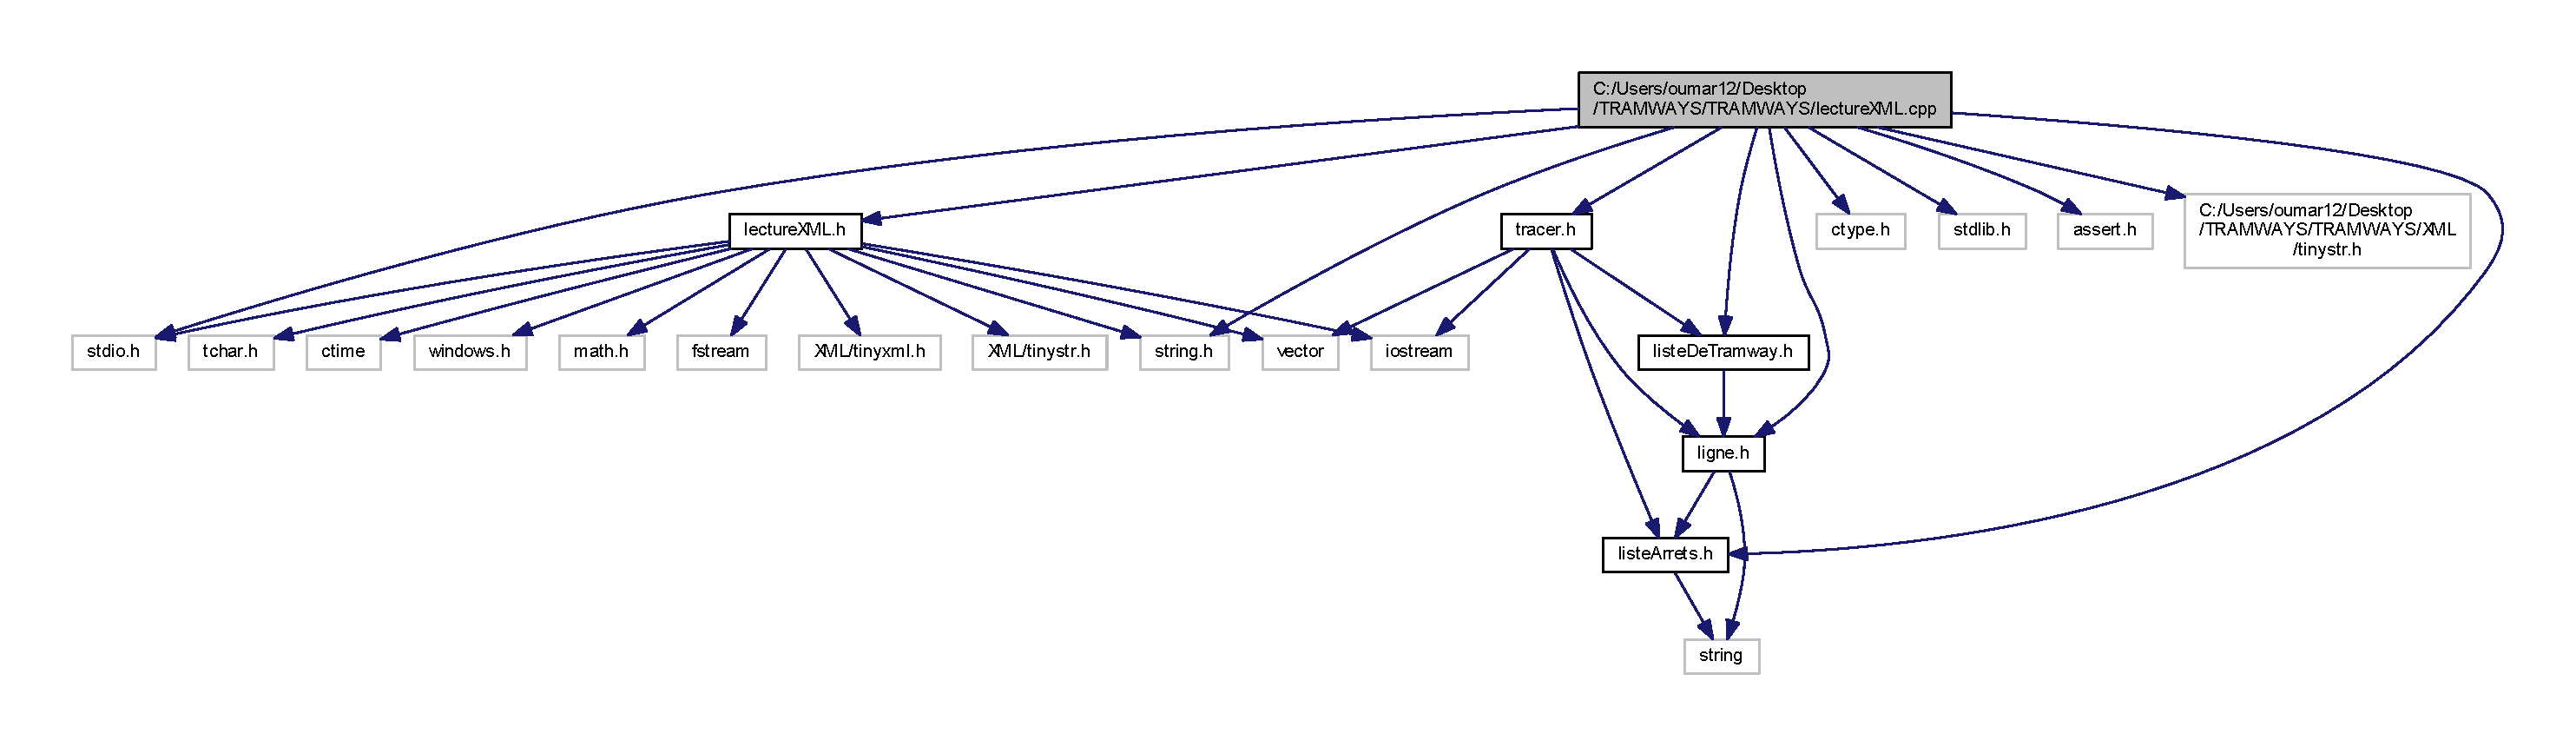
\includegraphics[width=350pt]{lecture_x_m_l_8cpp__incl}
\end{center}
\end{figure}

\hypertarget{lecture_x_m_l_8h}{}\section{C\+:/\+Users/oumar12/\+Desktop/\+T\+R\+A\+M\+W\+A\+Y\+S/\+T\+R\+A\+M\+W\+A\+Y\+S/lecture\+X\+ML.h File Reference}
\label{lecture_x_m_l_8h}\index{C\+:/\+Users/oumar12/\+Desktop/\+T\+R\+A\+M\+W\+A\+Y\+S/\+T\+R\+A\+M\+W\+A\+Y\+S/lecture\+X\+M\+L.\+h@{C\+:/\+Users/oumar12/\+Desktop/\+T\+R\+A\+M\+W\+A\+Y\+S/\+T\+R\+A\+M\+W\+A\+Y\+S/lecture\+X\+M\+L.\+h}}
{\ttfamily \#include $<$iostream$>$}\\*
{\ttfamily \#include $<$fstream$>$}\\*
{\ttfamily \#include \char`\"{}X\+M\+L/tinyxml.\+h\char`\"{}}\\*
{\ttfamily \#include \char`\"{}X\+M\+L/tinystr.\+h\char`\"{}}\\*
{\ttfamily \#include $<$stdio.\+h$>$}\\*
{\ttfamily \#include $<$tchar.\+h$>$}\\*
{\ttfamily \#include $<$string.\+h$>$}\\*
{\ttfamily \#include $<$ctime$>$}\\*
{\ttfamily \#include $<$windows.\+h$>$}\\*
{\ttfamily \#include $<$math.\+h$>$}\\*
{\ttfamily \#include $<$vector$>$}\\*
Include dependency graph for lecture\+X\+M\+L.\+h\+:
\nopagebreak
\begin{figure}[H]
\begin{center}
\leavevmode
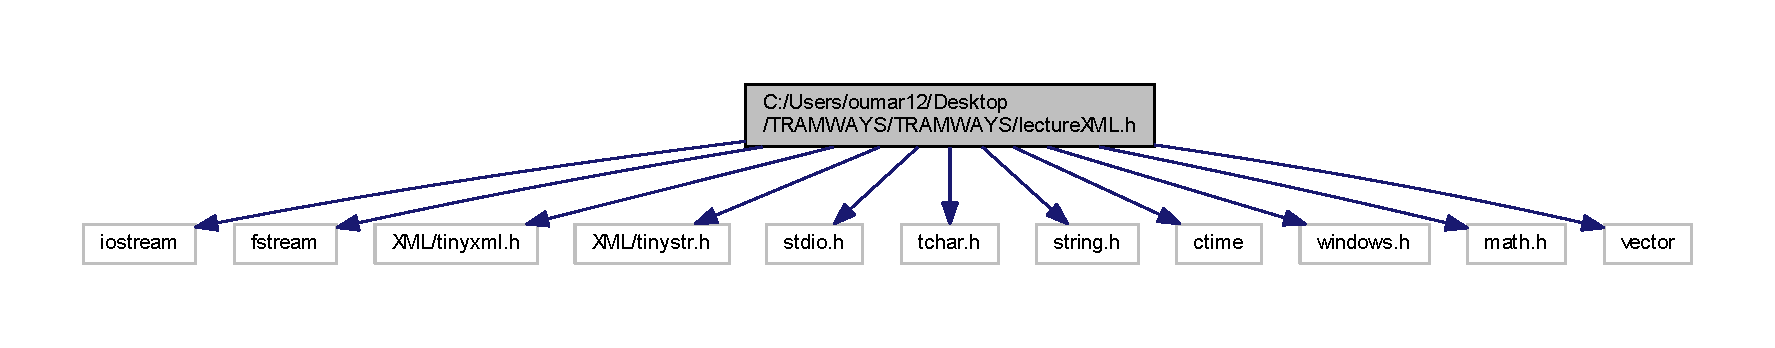
\includegraphics[width=350pt]{lecture_x_m_l_8h__incl}
\end{center}
\end{figure}
This graph shows which files directly or indirectly include this file\+:
\nopagebreak
\begin{figure}[H]
\begin{center}
\leavevmode
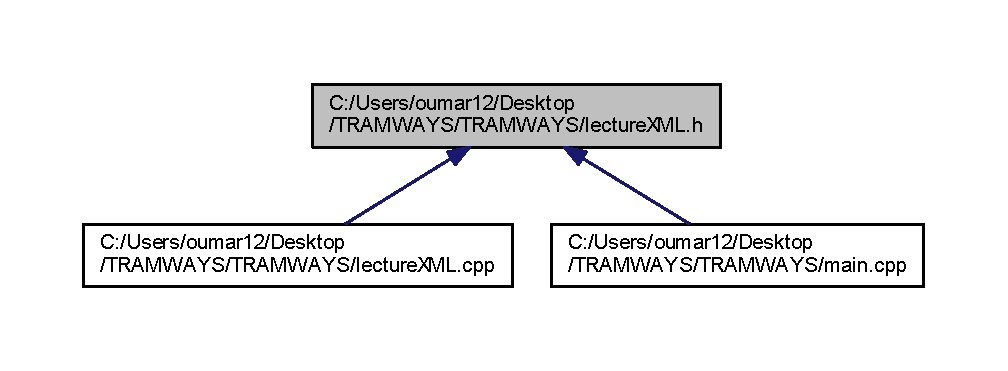
\includegraphics[width=350pt]{lecture_x_m_l_8h__dep__incl}
\end{center}
\end{figure}
\subsection*{Classes}
\begin{DoxyCompactItemize}
\item 
class \hyperlink{classlecture_x_m_l}{lecture\+X\+ML}
\end{DoxyCompactItemize}

\hypertarget{ligne_8cpp}{}\section{C\+:/\+Users/oumar12/\+Desktop/\+T\+R\+A\+M\+W\+A\+Y\+S/\+T\+R\+A\+M\+W\+A\+Y\+S/ligne.cpp File Reference}
\label{ligne_8cpp}\index{C\+:/\+Users/oumar12/\+Desktop/\+T\+R\+A\+M\+W\+A\+Y\+S/\+T\+R\+A\+M\+W\+A\+Y\+S/ligne.\+cpp@{C\+:/\+Users/oumar12/\+Desktop/\+T\+R\+A\+M\+W\+A\+Y\+S/\+T\+R\+A\+M\+W\+A\+Y\+S/ligne.\+cpp}}
{\ttfamily \#include $<$iostream$>$}\\*
{\ttfamily \#include $<$fstream$>$}\\*
{\ttfamily \#include $<$string$>$}\\*
{\ttfamily \#include \char`\"{}ligne.\+h\char`\"{}}\\*
Include dependency graph for ligne.\+cpp\+:
\nopagebreak
\begin{figure}[H]
\begin{center}
\leavevmode
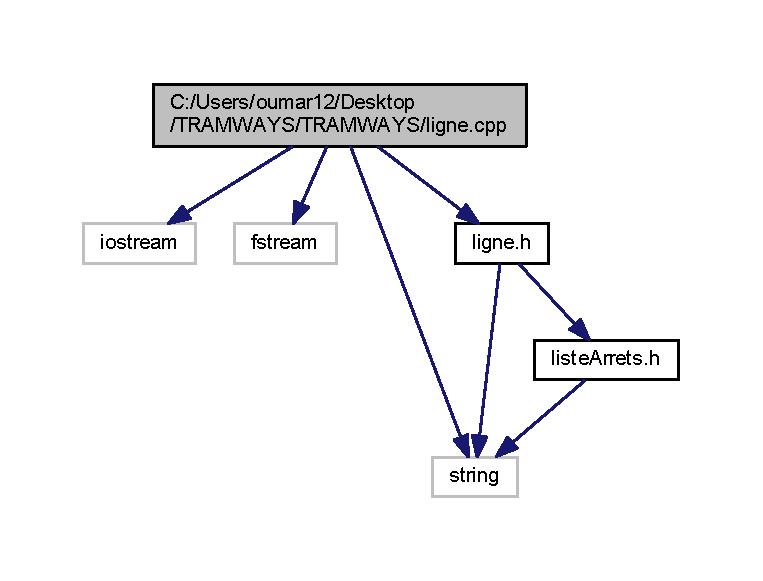
\includegraphics[width=350pt]{ligne_8cpp__incl}
\end{center}
\end{figure}

\hypertarget{ligne_8h}{}\section{C\+:/\+Users/oumar12/\+Desktop/\+T\+R\+A\+M\+W\+A\+Y\+S/\+T\+R\+A\+M\+W\+A\+Y\+S/ligne.h File Reference}
\label{ligne_8h}\index{C\+:/\+Users/oumar12/\+Desktop/\+T\+R\+A\+M\+W\+A\+Y\+S/\+T\+R\+A\+M\+W\+A\+Y\+S/ligne.\+h@{C\+:/\+Users/oumar12/\+Desktop/\+T\+R\+A\+M\+W\+A\+Y\+S/\+T\+R\+A\+M\+W\+A\+Y\+S/ligne.\+h}}
{\ttfamily \#include $<$string$>$}\\*
{\ttfamily \#include \char`\"{}liste\+Arrets.\+h\char`\"{}}\\*
Include dependency graph for ligne.\+h\+:
\nopagebreak
\begin{figure}[H]
\begin{center}
\leavevmode
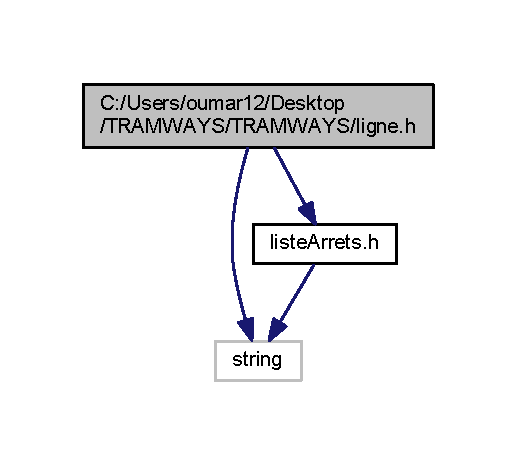
\includegraphics[width=248pt]{ligne_8h__incl}
\end{center}
\end{figure}
This graph shows which files directly or indirectly include this file\+:
\nopagebreak
\begin{figure}[H]
\begin{center}
\leavevmode
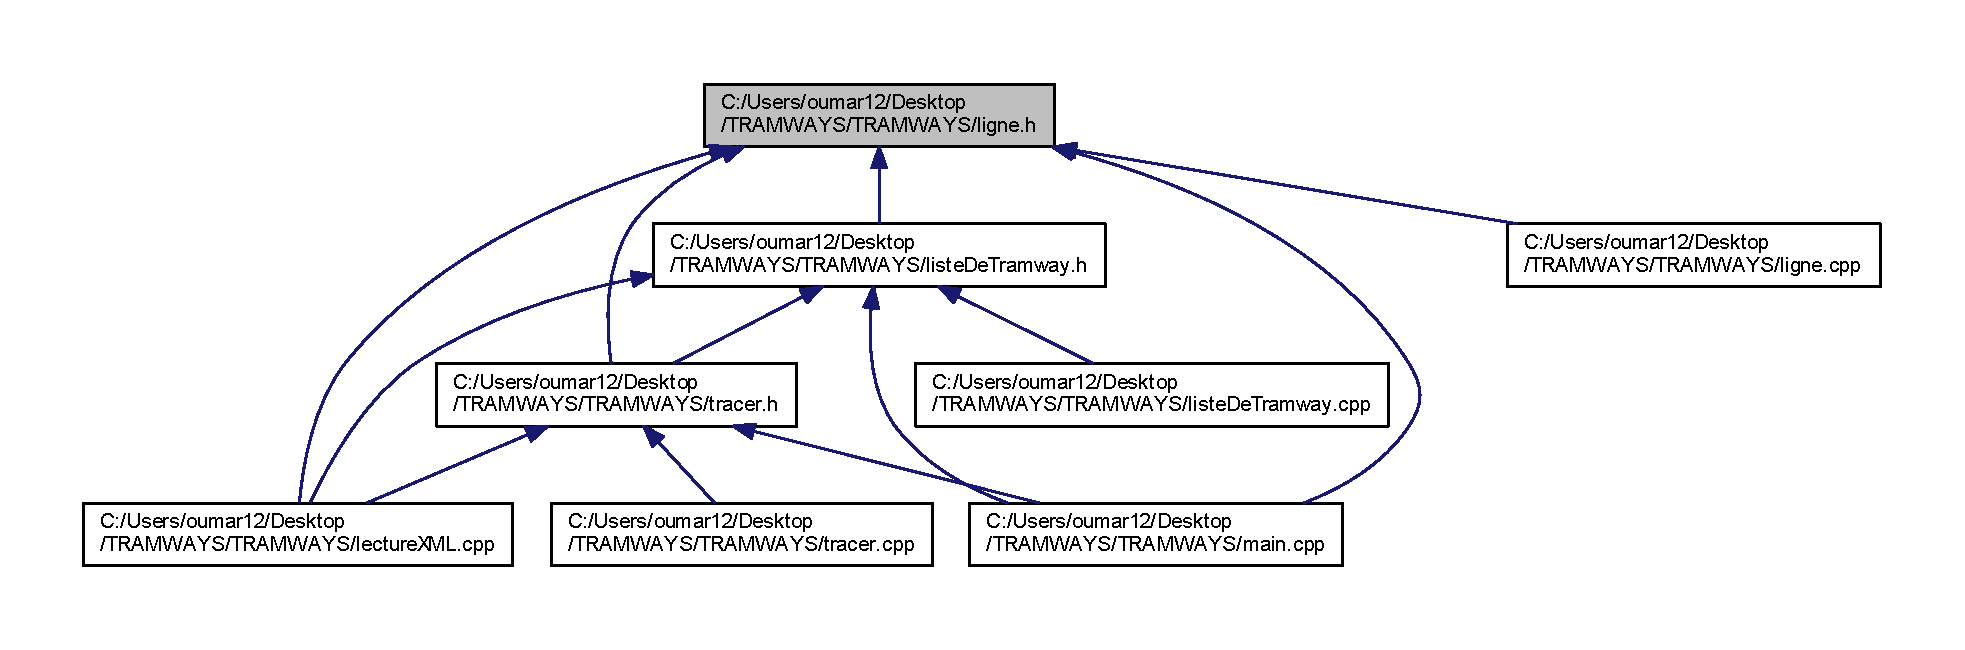
\includegraphics[width=350pt]{ligne_8h__dep__incl}
\end{center}
\end{figure}
\subsection*{Classes}
\begin{DoxyCompactItemize}
\item 
class \hyperlink{classligne}{ligne}
\end{DoxyCompactItemize}

\hypertarget{liste_arrets_8cpp}{}\section{C\+:/\+Users/oumar12/\+Desktop/\+T\+R\+A\+M\+W\+A\+Y\+S/\+T\+R\+A\+M\+W\+A\+Y\+S/liste\+Arrets.cpp File Reference}
\label{liste_arrets_8cpp}\index{C\+:/\+Users/oumar12/\+Desktop/\+T\+R\+A\+M\+W\+A\+Y\+S/\+T\+R\+A\+M\+W\+A\+Y\+S/liste\+Arrets.\+cpp@{C\+:/\+Users/oumar12/\+Desktop/\+T\+R\+A\+M\+W\+A\+Y\+S/\+T\+R\+A\+M\+W\+A\+Y\+S/liste\+Arrets.\+cpp}}
{\ttfamily \#include $<$iostream$>$}\\*
{\ttfamily \#include $<$fstream$>$}\\*
{\ttfamily \#include \char`\"{}liste\+Arrets.\+h\char`\"{}}\\*
Include dependency graph for liste\+Arrets.\+cpp\+:
\nopagebreak
\begin{figure}[H]
\begin{center}
\leavevmode
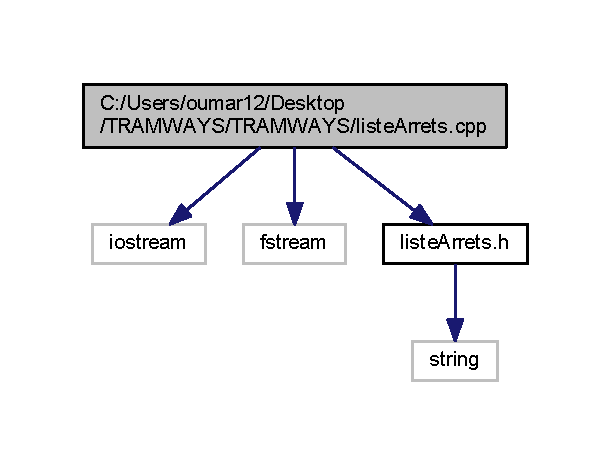
\includegraphics[width=293pt]{liste_arrets_8cpp__incl}
\end{center}
\end{figure}

\hypertarget{liste_arrets_8h}{}\section{C\+:/\+Users/oumar12/\+Desktop/\+T\+R\+A\+M\+W\+A\+Y\+S/\+T\+R\+A\+M\+W\+A\+Y\+S/liste\+Arrets.h File Reference}
\label{liste_arrets_8h}\index{C\+:/\+Users/oumar12/\+Desktop/\+T\+R\+A\+M\+W\+A\+Y\+S/\+T\+R\+A\+M\+W\+A\+Y\+S/liste\+Arrets.\+h@{C\+:/\+Users/oumar12/\+Desktop/\+T\+R\+A\+M\+W\+A\+Y\+S/\+T\+R\+A\+M\+W\+A\+Y\+S/liste\+Arrets.\+h}}
{\ttfamily \#include $<$string$>$}\\*
Include dependency graph for liste\+Arrets.\+h\+:
\nopagebreak
\begin{figure}[H]
\begin{center}
\leavevmode
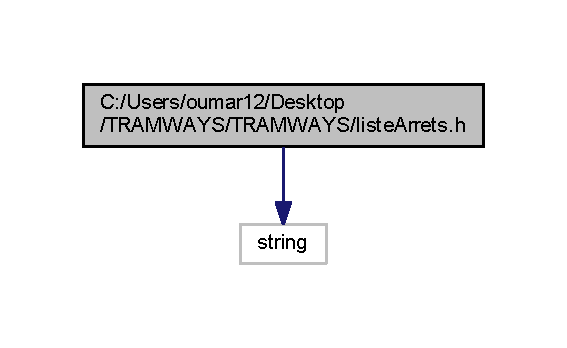
\includegraphics[width=272pt]{liste_arrets_8h__incl}
\end{center}
\end{figure}
This graph shows which files directly or indirectly include this file\+:
\nopagebreak
\begin{figure}[H]
\begin{center}
\leavevmode
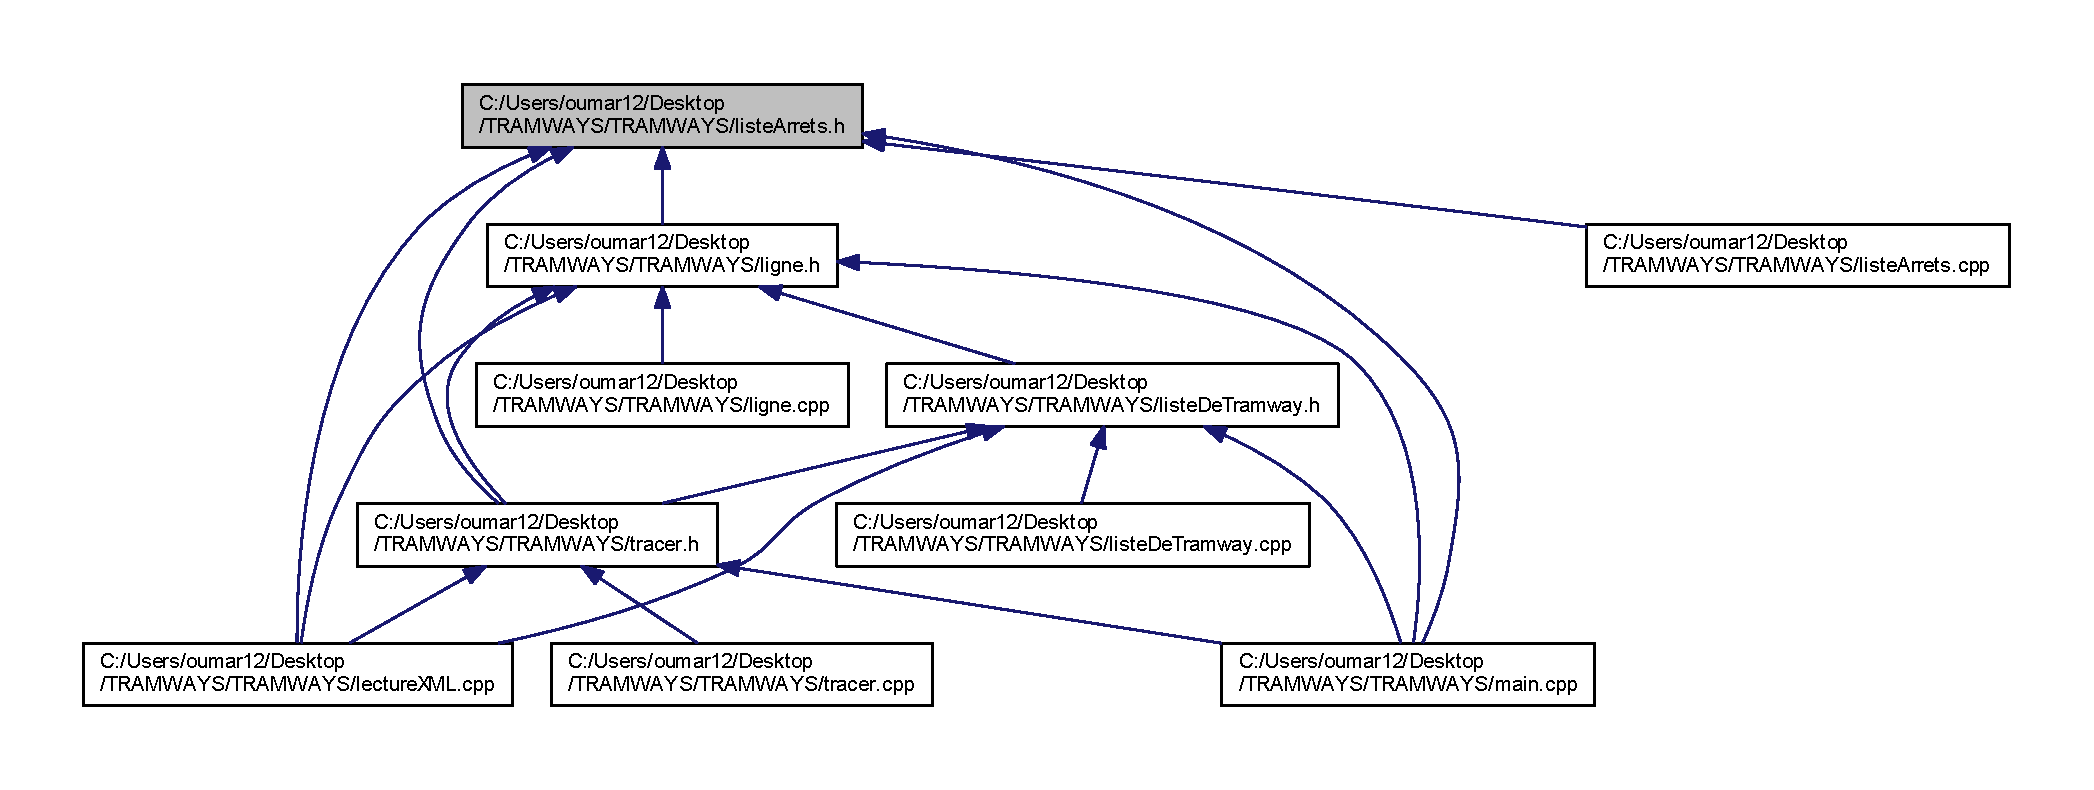
\includegraphics[width=350pt]{liste_arrets_8h__dep__incl}
\end{center}
\end{figure}
\subsection*{Classes}
\begin{DoxyCompactItemize}
\item 
class \hyperlink{classarret}{arret}
\item 
class \hyperlink{classliste_arrets}{liste\+Arrets}
\end{DoxyCompactItemize}

\hypertarget{liste_de_tramway_8cpp}{}\section{C\+:/\+Users/oumar12/\+Desktop/\+T\+R\+A\+M\+W\+A\+Y\+S/\+T\+R\+A\+M\+W\+A\+Y\+S/liste\+De\+Tramway.cpp File Reference}
\label{liste_de_tramway_8cpp}\index{C\+:/\+Users/oumar12/\+Desktop/\+T\+R\+A\+M\+W\+A\+Y\+S/\+T\+R\+A\+M\+W\+A\+Y\+S/liste\+De\+Tramway.\+cpp@{C\+:/\+Users/oumar12/\+Desktop/\+T\+R\+A\+M\+W\+A\+Y\+S/\+T\+R\+A\+M\+W\+A\+Y\+S/liste\+De\+Tramway.\+cpp}}
{\ttfamily \#include $<$iostream$>$}\\*
{\ttfamily \#include \char`\"{}liste\+De\+Tramway.\+h\char`\"{}}\\*
{\ttfamily \#include $<$cmath$>$}\\*
Include dependency graph for liste\+De\+Tramway.\+cpp\+:
\nopagebreak
\begin{figure}[H]
\begin{center}
\leavevmode
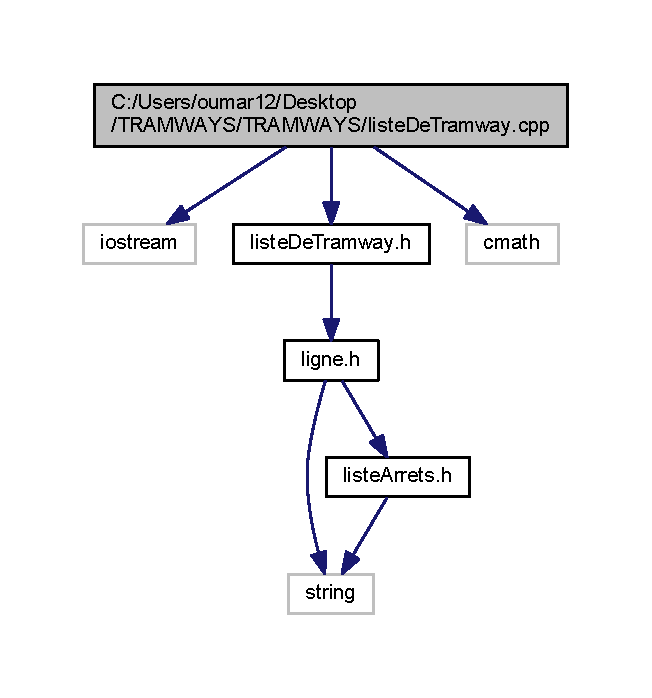
\includegraphics[width=313pt]{liste_de_tramway_8cpp__incl}
\end{center}
\end{figure}

\hypertarget{liste_de_tramway_8h}{}\section{C\+:/\+Users/oumar12/\+Desktop/\+T\+R\+A\+M\+W\+A\+Y\+S/\+T\+R\+A\+M\+W\+A\+Y\+S/liste\+De\+Tramway.h File Reference}
\label{liste_de_tramway_8h}\index{C\+:/\+Users/oumar12/\+Desktop/\+T\+R\+A\+M\+W\+A\+Y\+S/\+T\+R\+A\+M\+W\+A\+Y\+S/liste\+De\+Tramway.\+h@{C\+:/\+Users/oumar12/\+Desktop/\+T\+R\+A\+M\+W\+A\+Y\+S/\+T\+R\+A\+M\+W\+A\+Y\+S/liste\+De\+Tramway.\+h}}
{\ttfamily \#include \char`\"{}ligne.\+h\char`\"{}}\\*
Include dependency graph for liste\+De\+Tramway.\+h\+:
\nopagebreak
\begin{figure}[H]
\begin{center}
\leavevmode
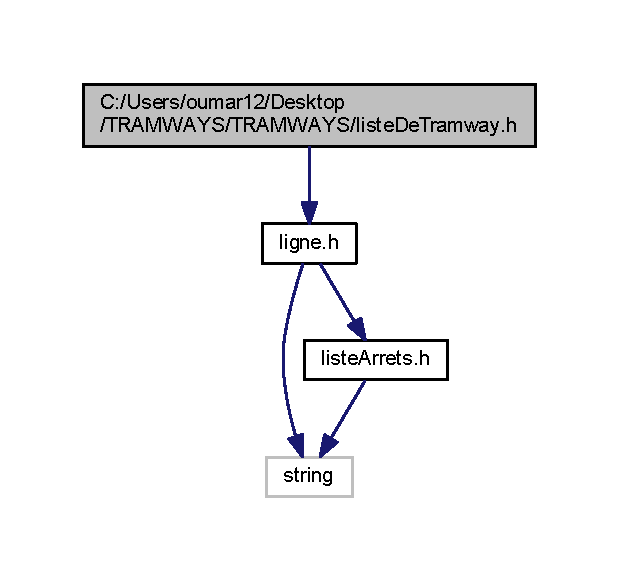
\includegraphics[width=297pt]{liste_de_tramway_8h__incl}
\end{center}
\end{figure}
This graph shows which files directly or indirectly include this file\+:
\nopagebreak
\begin{figure}[H]
\begin{center}
\leavevmode
\includegraphics[width=350pt]{liste_de_tramway_8h__dep__incl}
\end{center}
\end{figure}
\subsection*{Classes}
\begin{DoxyCompactItemize}
\item 
class \hyperlink{classtramway}{tramway}
\item 
class \hyperlink{classliste_de_trams}{liste\+De\+Trams}
\end{DoxyCompactItemize}

\hypertarget{main_8cpp}{}\section{C\+:/\+Users/oumar12/\+Desktop/\+T\+R\+A\+M\+W\+A\+Y\+S/\+T\+R\+A\+M\+W\+A\+Y\+S/main.cpp File Reference}
\label{main_8cpp}\index{C\+:/\+Users/oumar12/\+Desktop/\+T\+R\+A\+M\+W\+A\+Y\+S/\+T\+R\+A\+M\+W\+A\+Y\+S/main.\+cpp@{C\+:/\+Users/oumar12/\+Desktop/\+T\+R\+A\+M\+W\+A\+Y\+S/\+T\+R\+A\+M\+W\+A\+Y\+S/main.\+cpp}}
{\ttfamily \#include $<$iostream$>$}\\*
{\ttfamily \#include \char`\"{}liste\+De\+Tramway.\+h\char`\"{}}\\*
{\ttfamily \#include \char`\"{}liste\+Arrets.\+h\char`\"{}}\\*
{\ttfamily \#include \char`\"{}ligne.\+h\char`\"{}}\\*
{\ttfamily \#include \char`\"{}tracer.\+h\char`\"{}}\\*
{\ttfamily \#include \char`\"{}lecture\+X\+M\+L.\+h\char`\"{}}\\*
{\ttfamily \#include $<$windows.\+h$>$}\\*
{\ttfamily \#include \char`\"{}graphics.\+h\char`\"{}}\\*
Include dependency graph for main.\+cpp\+:
\nopagebreak
\begin{figure}[H]
\begin{center}
\leavevmode
\includegraphics[width=350pt]{main_8cpp__incl}
\end{center}
\end{figure}
\subsection*{Functions}
\begin{DoxyCompactItemize}
\item 
int \hyperlink{main_8cpp_a0ddf1224851353fc92bfbff6f499fa97}{main} (int argc, char $\ast$argv\mbox{[}$\,$\mbox{]})
\end{DoxyCompactItemize}


\subsection{Function Documentation}
\index{main.\+cpp@{main.\+cpp}!main@{main}}
\index{main@{main}!main.\+cpp@{main.\+cpp}}
\subsubsection[{\texorpdfstring{main(int argc, char $\ast$argv[])}{main(int argc, char *argv[])}}]{\setlength{\rightskip}{0pt plus 5cm}int main (
\begin{DoxyParamCaption}
\item[{int}]{argc, }
\item[{char $\ast$}]{argv\mbox{[}$\,$\mbox{]}}
\end{DoxyParamCaption}
)}\hypertarget{main_8cpp_a0ddf1224851353fc92bfbff6f499fa97}{}\label{main_8cpp_a0ddf1224851353fc92bfbff6f499fa97}

\hypertarget{tracer_8cpp}{}\section{C\+:/\+Users/oumar12/\+Desktop/\+T\+R\+A\+M\+W\+A\+Y\+S/\+T\+R\+A\+M\+W\+A\+Y\+S/tracer.cpp File Reference}
\label{tracer_8cpp}\index{C\+:/\+Users/oumar12/\+Desktop/\+T\+R\+A\+M\+W\+A\+Y\+S/\+T\+R\+A\+M\+W\+A\+Y\+S/tracer.\+cpp@{C\+:/\+Users/oumar12/\+Desktop/\+T\+R\+A\+M\+W\+A\+Y\+S/\+T\+R\+A\+M\+W\+A\+Y\+S/tracer.\+cpp}}
{\ttfamily \#include \char`\"{}graphics.\+h\char`\"{}}\\*
{\ttfamily \#include $<$iostream$>$}\\*
{\ttfamily \#include $<$ctime$>$}\\*
{\ttfamily \#include $<$tchar.\+h$>$}\\*
{\ttfamily \#include $<$math.\+h$>$}\\*
{\ttfamily \#include \char`\"{}tracer.\+h\char`\"{}}\\*
{\ttfamily \#include $<$windows.\+h$>$}\\*
Include dependency graph for tracer.\+cpp\+:
\nopagebreak
\begin{figure}[H]
\begin{center}
\leavevmode
\includegraphics[width=350pt]{tracer_8cpp__incl}
\end{center}
\end{figure}

\hypertarget{tracer_8h}{}\section{C\+:/\+Users/oumar12/\+Desktop/\+T\+R\+A\+M\+W\+A\+Y\+S/\+T\+R\+A\+M\+W\+A\+Y\+S/tracer.h File Reference}
\label{tracer_8h}\index{C\+:/\+Users/oumar12/\+Desktop/\+T\+R\+A\+M\+W\+A\+Y\+S/\+T\+R\+A\+M\+W\+A\+Y\+S/tracer.\+h@{C\+:/\+Users/oumar12/\+Desktop/\+T\+R\+A\+M\+W\+A\+Y\+S/\+T\+R\+A\+M\+W\+A\+Y\+S/tracer.\+h}}
{\ttfamily \#include $<$iostream$>$}\\*
{\ttfamily \#include $<$vector$>$}\\*
{\ttfamily \#include \char`\"{}liste\+Arrets.\+h\char`\"{}}\\*
{\ttfamily \#include \char`\"{}ligne.\+h\char`\"{}}\\*
{\ttfamily \#include \char`\"{}liste\+De\+Tramway.\+h\char`\"{}}\\*
Include dependency graph for tracer.\+h\+:
\nopagebreak
\begin{figure}[H]
\begin{center}
\leavevmode
\includegraphics[width=350pt]{tracer_8h__incl}
\end{center}
\end{figure}
This graph shows which files directly or indirectly include this file\+:
\nopagebreak
\begin{figure}[H]
\begin{center}
\leavevmode
\includegraphics[width=350pt]{tracer_8h__dep__incl}
\end{center}
\end{figure}
\subsection*{Classes}
\begin{DoxyCompactItemize}
\item 
class \hyperlink{classtracer}{tracer}
\end{DoxyCompactItemize}

%--- End generated contents ---

% Index
\backmatter
\newpage
\phantomsection
\clearemptydoublepage
\addcontentsline{toc}{chapter}{Index}
\printindex

\end{document}
